%\begin{savequote}[75mm]
%This is some random quote to start off the chapter.
%\qauthor{Firstname lastname}
%\end{savequote}

\chapter{Literature review}
To address the compound crises of climate and information, we must produce new knowledge and activate existing knowledge from various disciplines. Solutions to the climate crisis may already exist but remain hidden in the overwhelming amount of information available. To rethink how we integrate knowledge, we must take an interdisciplinary approach.

\section{Type of literature review}
Following Grant and Booth’s typology of reviews \citep[p. 91-108]{grant_typology_2009}, my thesis research uses mixed methods and a scoping review.

\subsection{Mixed methods review}
%\noindent \textbf{Mixed methods review} \\
As a mixed methods review, I combine quantitative and qualitative research from different fields. My research project is an example of how mixed methods reviews should be, by their nature, interdisciplinary, which means they analyze various disciplines. Drawing from philosophy, computer science, and mathematics, I examine a ``correlation between characteristics” to identify gaps in areas of literature \citep[p. 94]{grant_typology_2009}. In my research, I was unable to find studies, methods or platforms that propose or accomplish the following tasks simultaneously:
\begin{enumerate}
    \item[-] Distinguishing the various modalities of knowledge and ranks them by their expense, including distinct definitions between modes of Knowledge Activation, including Surfacing, Synthesis, Translation, and Production. The limited subtlety in this subject makes climate resilience research more costly than it needs to be. It is imperative to distinguish and quantify the expense of various modalities of Knowledge Activation by their expense to reduce unnecessary costs in climate resilience research.
\item[-] Distinguishing three-dimensional forms by the various ways they capture and reveal reasoning and other semantic relationships as layouts for text graphs and graph chunks. The limited research in this area restrains exploration of Visuospatial Knowledge Activation in various fields, including neuroscience, learning psychology, and design. Visuospatial models facilitate understanding because they capture and reveal reasoning and semantic relationships in text graph composition and graph chunks.
\item[-] Distinguishing how capturing and revealing semantic relationships in text graphs can be distinctly non-computational with the \textit{option} of being computational. In other words, I am pursuing solutions that do not impose but rather offer the option for computational analysis of texts and graphs (CATG), which keep humans in the loop (HITL). The limited distinction and combination of computational machine-driven and human-driven ‘manual’ methods in the visuospatial modes of Knowledge Production (a) hinders the use of valuable training data for LLMs that can support climate resilience research, (b) demonstrates that the practical applications of existing visuospatial modes of Knowledge Production lack a strong connection to research findings that indicate its value, and (c) limits the ways valuable technology can be used by climate resilience researchers. We must distinguish human-driven and machine-driven modes of VKA to take better advantage of each mode and the effectiveness of their combined use.  
\item[-] Deployment of contemporary tools for the non-computational Human Analysis of Texts and Graphs (HATG) that relies on manual placement of words and visual elements in three-dimensional space (e.g. Systemic Design, Systems Oriented Design, Systematic Combining, Boundary Critique). The limited options in this area prevent us from using the full range of our human ability to reason in visuospatial modes of Knowledge Activation and the optical opportunities beyond the restrictions of two-dimensional information representation. We must build better tools for non-computational HATG using manual placement in three-dimensional space to more fully apply the creative potential of human VKA beyond two-dimensional limits.
\item[-] Methods that use HATG to train algorithms or LLMs. We must drive research in this area to increase the impact of LLMs in climate resilience research and overall research. 
\end{enumerate}
\index[terms]{Visuospatial Knowledge Activation (VKA)} \index[terms]{Systemic Design} \index[terms]{Large Language Model (LLM)}
\index[terms]{Systematic Combining (SC)}
\index[terms]{Knowledge Production (KP)}
\index[terms]{composition}
\index[terms]{Systems Oriented Design (SOD)}
\index[terms]{Boundary Critique}
\index[terms]{climate resilience}

\subsection{Scoping review}
%\noindent \textbf{Scoping review} \\
For my scoping review, I used a keyword search across various databases, including the terms information visualization, visuospatial, personal knowledge management, digital scholarship, and others. 

To select the papers I read, I optimized for the depth of the coverage of each subject, opting for longer papers and publications whenever possible. I favoured primary research, which included more reflective pieces and experimental, qualitative, quantitative, and mixed-methods studies in various fields of mathematics and science, including systematic reviews. 

I aimed to assess the ``potential size and scope of available research” projects \citep[p. 95]{grant_typology_2009}. In doing so, I investigated whether any existing projects modelled the categorization of large groups of highly influential ideas in three-dimensional forms. Notably, I found only one example: Brian Sunter’s Wikipedia graphs \citep{sunter_organizing_2022, sunter_3d_2023}. 

I extended the scoping review method with a step recommended in systematic reviews, which often include a quality assessment step that inspired me to include recommendations for future research based on what remains unknown \citep[p. 95]{grant_typology_2009}. However, I cannot claim to propose what is \textit{not} known; only what I suggest \textit{may} be known. 

\section{Climate crisis: what is at stake}
Despite the misinformation about climate change, there is a nearly complete consensus that human causes are to blame \citep{Cook_2016,lynas_greater_2021}. According to Pörtner et al., none of the twenty ``2011–2020 Aichi biodiversity targets and none of the mileposts on climate trajectories intended to limit warming to 1.5°C have been met” \citep[p. 1]{portner_overcoming_2023}. The World Meteorological Organization (WMO) reports that the “past nine years, 2015–2023, were the nine warmest years on record” \citep[p. 3]{world_meteorological_organization_state_2024}. Despite this, greenhouse gas emissions continue to increase and “now exceed 55 billion tonnes of carbon dioxide equivalents” per year \citep[p. 1]{portner_overcoming_2023}. Critical life-saving targets have not been met, and yet humanity continues to increase its greenhouse gas emissions.

Our outlook is bleak if we do not work together. If the root causes of climate change and biodiversity loss are not met with a plan of action, global sustainability targets will continue to fail. We need radical collective action that addresses ``climate, biodiversity, and society” together, which ``can help to avoid dangerous trade-offs and maximize cobenefits for humankind” \citep[p. 1]{portner_overcoming_2023}. To ensure a livable future, we urgently need bold policies that better steward ``interlinked human, ecosystem, and planetary health” through coordinated social systems, institutions, and governance at local and global levels \citep[p. 1]{portner_overcoming_2023}. If we want a chance of avoiding much larger consequences to global warming, many more of us need to think more critically about our relationship to the larger web of life and its ecosystems. 

New large-scale solutions are required, and fast. The changes required to achieve the aims of the United Nations Framework Convention on Climate Change (UNCCC), the Convention on Biological Diversity (CBD), and the United Nations (UN) 2030 Agenda for Sustainable Development and its Sustainable Development Goals ``will rely on far-reaching mobilization and transformation actions of a type never before attempted” \citep[p. 8]{portner_overcoming_2023}. We need new solutions for global warming because we need to ``keep global warming below 1.5°C [...] to secure a livable future” \citep[p. 8]{portner_overcoming_2023}. 

To develop solutions that address the many aspects involved in global warming by working together across differences of disciplinary expertise is inevitable. In this way, this thesis is an investigation of how the development of technological research accelerators could allow us to find and implement more and better ways of stewarding our web of life. 



\section{Sociopolitics}
Clinging to the hope that we are yet discussing humanities and not posthumanities, I posit that the climate crisis is a crisis of understanding, institutionally and socially. 

%\noindent \textbf{Climate-related social change} \\
Applied climate-related understandings inevitably need to escalate the rate of collective social transformation if we want to minimize loss of life. 

Pörtner et al.'s review summary on societal impacts of sustainability polycrisis uses the term “social tipping” to refer to targeted interventions that cause self-reinforcing momentum ``with positive impacts on climate, biodiversity and human well-being" \citep[p. 7]{portner_overcoming_2023}. Building tools for managing complexity and inter/multi/trans-disciplinary research can identify social tipping interventions that are ``integrated and multifunctional" \citep[p. 1]{portner_overcoming_2023}, in and beyond social structures like governments and universities.


Social tipping as a shift in understanding is no small feat: “Activating such social tipping interventions necessarily involves a shift of individual and collectively shared social values away from individualism and materialism to principles such as responsibility, stewardship, and justice” \citep[p. 7]{portner_overcoming_2023}. Nonetheless, the more we do well, the more we will want to do well: “This vision of inclusive, integrative, and adaptive decision-making can overcome societal and political inertia” \citep[p. 8]{portner_overcoming_2023}. These solutions can “help society to avoid crossing biophysical tipping points and their worst impacts,” while also contributing to a “more just and sustainable world” \citep[p. 8]{portner_overcoming_2023}. Social tipping towards sustainability will only be possible as an initiative of climate resilience if we collectively shift our baseline values. This includes a shift to de-emphasize individualism towards collective well-being and responsibility. A shift like this carries the hope of catalyzing a virtuous cycle that overcomes the inertia of social and political stratification and marginalization in a way that helps mitigate environmental catastrophe. 
\index[terms]{climate resilience}

We risk squandering our limited chances to shift away from siloed approaches that, as Pörtner et al. claim, reinforce sociopolitical inertia, materialism, and individualism \citep[p. 7]{portner_overcoming_2023}. Pörtner et al. identify two notable climate policy gatherings that exemplify these policy nimbleness limitations, the United Nations Framework Convention on Climate Change (UNFCCC) and the Convention on Biological Diversity (CBD), which are often dominated by siloed approaches \citep[p. 7]{portner_overcoming_2023}. If we want to improve our global collaboration frameworks, we have to nurture the relationships and build the tools that bring about just, ``inclusive, integrative and adaptive decision-making" across policy sectors and solutions with ``cobenefits in terms of sustainable development" \citep[p. 7-8]{portner_overcoming_2023}. The impact of information technology innovation can fundamentally improve the sustainability of governance needs by improving collaboration across sectors. 

Coming to the defence of the most vulnerable and systemically oppressed is limited by the barriers to social tipping, and other forms of integrated coherence of cross-sectoral, multi-actor, multi-scale cooperation and policy \citep[p. 7]{portner_overcoming_2023}. 

Rapid action is required, “which entails transformative change through transformative governance” \citep[p. 7]{portner_overcoming_2023}. To echo Pörtner et al., rapid action in governance draws “on collaborative solutions across integrated systems, involves” diverse actors and values “about nature, engages different knowledge systems through more equitable approaches, and adaptively manages complex interactions” \citep[p. 7]{portner_overcoming_2023}. Collaborative solutions innovation can benefit all relational structures.


For the sake of the preservation of life, de-ecologized profits-centric economic and political frameworks must be named and challenged for acting against our collective body of life. Timothy Morton observes: ``Since its beginnings, capitalism has used war and catastrophe to reinvent itself. The current catastrophe is no exception. We should reject the false choice between the “politics of possibility” and a ``return to nature.” Instead, let's use this moment to imagine what sort of noncapitalist society we want” \citep[p. 133]{morton_ecological_2012}. This includes redefining the politics of computer production ``in the face of combined corporate and state power” \citep[p. 1]{chan_politics_2013}. As it stands, the domination of digital technology perpetuates imperialism \citep[p. 1]{kwet_digital_2018}, child labour at its worst \citep{amnesty_international_this_2016}, and formidable health hazards to children and pregnant parents caused by e-waste \citep{heacock_e-waste_2016}. The ecological crisis demands a re-making of economic and societal structures to challenge the ways technology perpetuates imperialism, labour exploitation, and environmental harm.
\index[people]{Morton, Timothy}


We must ``imagine collectivity rather than community—groups formed by choice rather than by necessity” \citep[p. 135]{morton_ecological_2012}. Morton asserts: “We have barely become conscious that we have been terraforming Earth all along. Now we have the chance to face up to this fact and to our coexistence with all beings” \citep[p. 133]{morton_ecological_2012}. In some ways, Morton's dedication in \textit{Hyperobjects} \citep[p. v]{morton_hyperobjects_2013} ``To my extended families" \footnote{Morton's dedication in \textit{Hyperobjects} \citep[p. v]{morton_hyperobjects_2013}, ``To my extended families", inspired my dedication statement in this thesis.} extends the notion of family beyond chosen family to include all beings in a heartbroken plea against humanity's destruction.
\index[people]{Morton, Timothy}
\index[terms]{hyperobject}


Developing information technology and its applied systemic interventions, like social tipping in the context of the climate hyperobject, can help lessen barriers in our necessary collective work in the interconnected problems of the environment, society, and economy. Notwithstanding the challenges of misinformation and disinformation caused by human machinations and AI hallucinations, global warming is a crisis of understanding. Herein lies the critical role of information and how it becomes Visuospatial Knowledge Activation as the bridge between the dangers we are in and the discovery of better solutions.
\index[terms]{Visuospatial Knowledge Activation (VKA)}



\section{Cognition}
\subsection{Information overload}
The unmanaged overflow of research adds to the difficulty of facing global warming. Terms related to \textit{information overload} are outlined by Eppler and Mengis \citep[p. 326]{eppler_concept_2004}, and include \textit{cognitive overload} \citep{vollmann_cutting_1991}, \textit{sensory overload} \citep{lipowski_sensory_1975}, \textit{communication overload} \citep{meier_communications_1963}, \textit{knowledge overload} \citep{hunt_medical_1997}, and \textit{information fatigue syndrome} \citep{wurman_information_2001}. 


The relevance of information overload to Knowledge Production is not new. Bawden and Robinson note that overload was mentioned by name as a problem at the Royal Society’s Scientific Information Conference in 1948 \citep[p. 183]{bawden_dark_2009}. Maurice Line is quoted as commenting: ``Not for the first time in history, but more acutely than every before, there was a fear that scientists would be overwhelmed, that they would be no longer able to control the vast amounts of potentially relevant material that were pouring forth from the world's presses, that science itself was under threat” \citep[p. 183]{bawden_dark_2009}. Information overload and the difficulty of managing the vast amount of potentially relevant material is not a new challenge, but the rate and scale at which new information is produced and made available pose an increasingly serious challenge to how we come to understandings at a highly critical time. This complex of problems can be faced with new strategies and tools.
\index[terms]{Knowledge Production (KP)}


\subsection{Hyperobjects}
As complex as the question of information is, the question of information overload about the climate crisis is, of course, much larger. In \textit{The ecological thought} (2012), Timothy Morton conveys this fearsome scope of being. Morton coins the term hyperobjects to mean ``things that are massively distributed in time and space relative to humans” \citep[p. 1]{morton_hyperobjects_2013}, global warming being one of them. 
\index[people]{Morton, Timothy}
\index[terms]{hyperobject}



Morton portends: ``Hyperobjects invoke a terror beyond the sublime, cutting deeper than conventional religious fear. A massive cathedral dome, the mystery of a stone circle, have nothing on the sheer existence of hyperobjects” \citep[p. 131]{morton_ecological_2012}. 
\index[people]{Morton, Timothy}
\index[terms]{hyperobject}


Morton forebodes that, in addition to global warming, hyperobjects like Styrofoam and plutonium will be part of the lasting human legacy. These materials will outlast current social and biological forms, the same way plastic takeout boxes last for hundreds of years, and plutonium remains for thousands, longer than Stonehenge has existed \citep[p. 130]{morton_ecological_2012}. Morton posits that hyperobjects, such as global warming and enduring pollutants, evoke a uniquely modern terror by existing on scales that dwarf human comprehension.
\index[people]{Morton, Timothy}
\index[terms]{hyperobject}

The illusion of current AI as a generator of knowledge would seem to elevate it to an authoritative position as a potential saviour in the climate crisis hyperobject. The possibility of mechanical agency notwithstanding, the set of semantic relationships that any AI uses to generate media is the result of constructions used in every step of its design, from algorithms to the words captured as tokens and stored in vector graph form. 

To encounter understandings, we have to set definitions to break them, and iterate constantly. If humanity is to ever encounter, re-encounter, and nurture hyperobject relationships, semantic and otherwise, that better honour the wide web of being and provide the relief of direction for even the short while of centuries, we must continue to brave vertiginous conditions of terror, in the hope of perhaps re-encountering wonder.

\index[terms]{Knowledge Production (KP)}
\index[terms]{hyperobject}




\subsection{Coping by using design}
%\noindent \textbf{Coping by using design} \\
Conversely to \textit{overload}, methods exist for \textit{coping} with more complex information visually. Considering the cognitive overload of the climate hyperobject, I turn here to the practice of design, specifically Systems Oriented Design (SOD). SOD is a confluence of various graphing methodologies brought together by Birger Sevaldson which hones ``the ability to cope with much larger amounts of information” \citep[p. 34]{sevaldson_designing_2022}. Sevaldson asserts that visualization ``is simply the best way to understand complex issues” \citep[p. 34]{sevaldson_designing_2022}. They stress the designer’s ``inherent ability to work with complexity” and their ``advantage in visual reasoning and thinking” \citep[p. 34]{sevaldson_designing_2022}. If SOD helps manage complexity, it can play a role in facing global warming. 
\index[terms]{hyperobject}
\index[terms]{Systems Oriented Design (SOD)}















\subsection{The visuospatial}
%\noindent \textbf{The visuospatial} \\

Barbara Tversky’s work in the neuroscience of the visuospatial examines the implications of how brains evolved to handle position in space before they evolved the ability to handle language. In fact, Tversky claims that ``spatial thinking is the foundation of all thought” \citep{tversky_barbara_2022}.

Tversky's work relates to and builds on the research by John O’Keefe, May-Britt Moser, and Edvard I. Moser which was awarded the 2014 Nobel Prize in Physiology or Medicine for their ``discoveries of cells that constitute a positioning system in the brain" \citep{fyhn_spatial_2004,hafting_microstructure_2005,okeefe_hippocampus_1971,okeefe_place_1976,okeefe_hippocampus_1978,the_nobel_committee_for_physiology_or_medicine_nobel_2014,nobel_prize_outreach_nobel_2014,sargolini_conjunctive_2006}.

Among her many insights, Tversky found that humans use the body and gestures ``to ‘externalize’ thought when we can’t articulate it yet." She has also observed that we remember better when we use spatial gestures. More specifically to human spacial signification, Tversky has found that ``spatial metaphors encode emotion, power, morality—often as vertical hierarchies" \citep{tversky_barbara_2022}. It would not be an exaggeration to claim that human sense of place in space precedes and fundamentally shapes communication, language, and reason.


\index[people]{Tversky, Barbara}
\index[people]{O’Keefe, John}
\index[people]{Moser, May-Britt}
\index[people]{Moser, Edvard I.}




\section{Ideas and their ‘place’ of origin}

In theological terms, the idea of \textit{other-origin} can be attributed to a transcendental agent which can choose to reveal itself or not. In the \textit{The Sacred and the Profane}, Mircea Eliade proposes that humanity ``becomes aware of the sacred'' because ``\textit{something sacred shows itself to us}” as being ``of a wholly different order, a reality that does not belong to our world, in objects that are an integral part of our natural ``profane” world”. Eliade uses the term hierophany to refer to this ``\textit{act of manifestation of the sacred}” \citep[p. 11]{eliade_sacred_1987}.\footnote{Italics in this paragraph were used to conserve Eliade's formatting.}

Eliade proposes that the history of religions is made up of ``a great number of hierophanies, by manifestations of sacred realities” \citep[p. 11]{eliade_sacred_1987}. For Eliade, ``the supreme hierophany" is the Christian incarnation, in which a supreme God manifests as a human \citep[p. 11]{eliade_sacred_1987}, or how stated written in \textit{John} 1:14 as ``the Word became flesh" \citep [p. 193]{ridling_bible_1989}. Eliade designates a lower tier to ``elementary hierophany", which is when the sacred manifests in an ``ordinary object" like a tree or a stone \citep[p. 11]{eliade_sacred_1987}. I fear that the operationalization of interpretations that conceive of humanity as so precariously high and away other forms of being has lead many to irrecoverably forget human contingency and vulnerability in the broader entanglement of life.

\index[people]{Eliade, Mircea}
\index[terms]{Indigeneity}


In philosophical terms, Michel Foucault argues that Immanuel Kant made it possible to conceive of representation, and represented ideas, as being from an origin other than representation itself \citep{gutting_michel_2022}. Kant questioned ``whether ideas do in fact represent their objects and, if so, how (in virtue of what) they do so” \citep{gutting_michel_2022}. However, this certainly does not constitute that representation has \textit{nothing} to do with knowledge \citep{gutting_michel_2022}. In fact, constructed methods of Knowledge Production remain examples of how ``some (or even all) knowledge still essentially involved ideas’ representing objects” \citep{gutting_michel_2022}.
\index[people]{Foucault, Michel}
\index[people]{Kant, Immanuel}
\index[terms]{Knowledge Production (KP)}




\section{Language and knowledge}
In linguistics, structuralism upholds that ``a language is a self-contained relational structure, the elements of which derive their existence and their value from their distribution and oppositions in texts or discourse” \citep{britannica_structuralism_2024}. In contrast, poststructuralism holds that ``language is not a transparent medium that connects one directly with a “truth” or “reality” outside it but rather a structure or code, whose parts derive their meaning from their contrast with one another and not from any connection with an outside world” \citep{britannica_poststructuralism_2024}. Writers associated with poststructuralism often include Roland Barthes and Michel Foucault. 
\index[people]{Barthes, Roland}
\index[people]{Foucault, Michel}

Terry Eagleton echoes Barthes’s description of the shift in thinking from structuralism to poststructuralism as involving ``a movement from `work’ to `text’” \citetext{\citealp[p. 155]{barthes_image_1977}; \citealp[p. 120]{eagleton_literary_2006}}. Eagleton elaborates: ``It is a shift from seeing the poem or novel as a closed entity, equipped with definite meanings which it is the critic's task to decipher, to seeing it as irreducibly plural, an endless play of signifiers which can never be finally nailed down to a single centre, essence or meaning" \citep[p. 120]{eagleton_literary_2006}. Drucker indicates that the ``shift to expressive metrics and graphics” is crucial in moving from ``\textit{expression of constructed, interpretative information}” to ``\textit{constructed expression of perceived phenomena}” \citep[p. 130]{drucker_graphesis_2014}. Drucker's post-structuralist posture of interpretation supports Kant's critique of ideas as ``the unproblematic vehicles of knowledge" \citep{gutting_michel_2022}. Herein lies the critical role of the network graph as a construction for denoting the decentralized meaning of ideas using a greater diversity of non-alphabetical signifiers like point, line, and glyph.
\index[people]{Drucker, Johanna}
\index[people]{Barthes, Roland}
\index[people]{Eagleton, Terry}

Drucker's distinction between \textit{data} from \textit{capta}, as briefly introduced earlier, defines \textit{capta}, ``not an expression of idiosyncracy, emotion, or individual quirks, but a systematic expression of information understood as constructed, as phenomena perceived according to principles of observer-dependent interpretation” \citep[p. 131]{drucker_graphesis_2014}. Interpretation in this sense involves more than just ``constructedness and inflection” \citep[p. 130]{drucker_graphesis_2014}. Drucker emphasizes that working with capta requires understanding every metric "as a factor of X," where X represents a particular perspective, goal, assumption, presumption, or even just an established convention \citep[p. 131]{drucker_graphesis_2014}. By ``qualifying any metric as a factor of some condition, the character of the ``information” shifts from self-evident ``fact” [, or \textit{data},] to constructed interpretation motivated by a human agenda [ie. capta]” \citep[p. 131]{drucker_graphesis_2014}. Drucker challenges the notion of objective data, proposing instead the concept of \textit{capta} to emphasize how all information is constructed with observer-dependent interpretation and, as such, should be understood as a product of specific viewpoints rather than as self-evident facts.
\index[terms]{capta}
\index[terms]{data}
\index[people]{Drucker, Johanna}











\subsection{Risks and opportunities of expanding narrow language}
We turn here from a philosophical perspective to a more practical and linguistic scope. Specifically, cyberneticist Paul Pangaro’s work on language in organizations is synthesized in his conversational model of co-evolutionary design. Pangaro examines conversation by building on influences from Hugh Dubberly, Heinz von Foerster, Michael C. Geoghegan, and Gordon Pask to develop his model of co-evolutionary design \citep{pangaro_designing_2017}. In Pangaro’s model, conversation is used to iterate and evaluate across four phases: (a) ``to agree on goals", (b) to ``design the designing”, or in other words, to design ``a new space of possibilities” (c) ``to create new language", (d) ``to agree on means", back to (a), and so on \citep[p. 156]{pangaro_design_2011}. Pangaro’s model emphasizes conversation as a cyclical tool for organizational innovation and regeneration.
\index[people]{Pangaro, Paul}

To call in an equity-driven orientation for the linguistic work of information practice, I will expand the scope of point ``A” in Pangaro’s conversational model, ``Conversation to Agree on Goals” \citep[p. 156]{pangaro_design_2011}. Antionette D. Carroll and her collaborators at Creative Reaction Labs have developed a guide for Equity-Centred Community Design (ECCD), which charges the conversational component of Pangaro’s co-evolutionary design with an ethos of justice-oriented intersectional co-creative solidarity. Creative Reaction Labs define ``language setting” as developing ``agreed upon definitions for any recurring terms you will use throughout your work” in ECCD \citep[p. 8-11]{creative_reaction_lab_equity-centered_2018}. I will later propose Symbol-setting as a semiotic expansion of language setting in collaborative Knowledge Production.
\index[people]{Pangaro, Paul}
\index[people]{Carroll, Antionette D.}
\index[terms]{Knowledge Production (KP)}
\index[terms]{Symbol-setting}


I return here to Pangaro and his 2011 presentation for the MIT Design and Computation Group, where he presented his ``Notes on the Role of \textbf{Leadership and Language} in Regenerating Organizations” \citep[p. 142]{pangaro_design_2011}\footnote{Bolded text in quotes of Paul Pangaro does not represent added emphasis and was added to match his presentation formatting.}. Pangaro offers that ``an organization is its \textbf{language}” \citep[p. 143]{pangaro_design_2011}. He proposes that an organization is made its linguistic interchange- ``who talks to whom, about what” \citep[p. 143]{pangaro_design_2011}. The organization is regenerated by conversation by leading from agreement to transaction \citep[p. 143]{pangaro_design_2011}.
\index[people]{Pangaro, Paul}

Pangaro presented the risks and opportunities specificity as follows. The opportunity lies in how ``narrowing \textbf{language} increases efficiency” \citep[p. 144]{pangaro_design_2011}. However, the growth of organizational jargon developed ``to solve specific problems” leads to an overly narrow scope of communication over time \citep[p. 144]{pangaro_design_2011}. ``Narrowing \textbf{language} also increases ignorance” \citep[p. 146]{pangaro_design_2011}. An organization’s specialized jargon, while efficient for managing very short-term business operations, can become a barrier to innovation in “research, new discoveries, new approaches." We all face the issue of recognizing our own limitations: ``we do not know that we do not know" and thinking we know limits our learning \citep[p. 146]{pangaro_design_2011}. ``Developed as a tool to increase efficiencies, the organization's language, paradoxically, becomes a trap” \citep[p. 146]{pangaro_design_2011}. Overall, Pangaro points to the ongoing condition of learning required so that organizations can recognize innovation and adapt. \index[people]{Pangaro, Paul}

Birger Sevaldson might frame Pangaro’s narrowing of language as the problem of defaulting to simplification. As a paradigm that is widely ``regarded as positive in our culture”, Sevaldson cites examples from management and philosophy of science like the administrative tropes to ``keep it simple" and ``Occam’s razor” \citep[p. 98]{sevaldson_designing_2022}. Sevaldson offers that danger of “modernist simplification” is that it attempts to ``remove all symbolism and expression from design, and reduce it to its ``essence”" \citep[p. 98]{sevaldson_designing_2022}. Sevaldson stresses that it ``is not possible to reduce human life to such simplifications, nor is it possible to rid the meaning, values, and symbols from design without losing out on the richness of our culture” \citep[p. 98]{sevaldson_designing_2022}. The dynamic described by Pangaro’s ``narrowing of language” and by Sevaldson as oversimplification characterizes the disciplinary siloing which causes researchers to lose out on rich semantic depth.
\index[people]{Pangaro, Paul}

Conversely, and returning to Pangaro, ``expanding \textbf{language} increases opportunity. The conversations necessary for generating new opportunities come from the outside system. For an organization to survive, it must be able to acquire new, relevant language domains” \citep[p. 147]{pangaro_design_2011} Pangaro also proposes that ``to regenerate, an organization creates a new \textbf{language}. To support an organization’s future viability, effective decision makers actively introduce change into the system. They do so by generating new language that appropriate groups in the organization come to understand and embrace. This new language does not overtly challenge the pre-existing, efficient system, but rather creates new distinctions and supportive relationships” \citep[p. 148]{pangaro_design_2011}. In short, Pangaro argues that organizational regeneration depends on incorporating external language domains while engaging in the difficult task of introducing change that supports existing systems. 
\index[people]{Pangaro, Paul}


Sevaldson and P.W. Anderson discuss the epistemological risks of narrowing and expanding language and its impact on interdisciplinarity. Sevaldson claims that ``adding up of elements changes the interplay between them so that new levels of interpretation are needed for each level of complexity” \citep[p. 99]{sevaldson_designing_2022}. Anderson explains further that the reductionist scientific approach, while powerful for understanding ``simple fundamental laws does not imply the ability to start from those laws and reconstruct the universe” \citetext{\citealp[p. 393]{anderson_more_1972}; \citealp[p. 99]{sevaldson_designing_2022}}. In systems terms, I would paraphrase that understanding patterns within a model does not provide a complete picture of a complex system. As complexity increases, new laws and concepts can be observed ``requiring inspiration and creativity" to an equally great degree of the previous simpler stage of understanding \citetext{\citealp[p. 393]{anderson_more_1972}; \citealp[p. 99]{sevaldson_designing_2022}}.

Sevaldson wrote that the ``contradiction [sic.] between arts and science are constructed and have their roots in an old dichotomy between those fields. In design discourse, the arts are often dismissed as being intuitive, creative, and based on metaphors, etc. But intuition, creativity, and metaphors are all part of science. This dichotomy between art and science is relatively new and should not be taken as a given. There is no logic that moving away from art will make design more scientific” \citep[p. 159]{sevaldson_designing_2022}. As P.W. Anderson wrote, ``we must all start with a reductionism” \citep[p. 394]{anderson_more_1972}, but this does not preclude integration of systems, ideas, and methods, and even disciplines. 

P.W. Anderson's perspective on levels of complexity in relation to disciplinary uniqueness emphasizes the differentiation of methods. He writes: ``Psychology is not applied biology, nor is biology applied chemistry” \citep[p. 393]{anderson_more_1972}. Conversely, in 1999, Wilson proposed that a convergence of disciplinary integration from the natural sciences toward the social sciences was not only possible but underway \citep[p. 208]{wilson_consilience_1999}. Wilson highlighted the following four examples: first, cognitive neuroscience, drawing on cognitive psychology to “solve the mystery of conscious thought” \citep[p. 208-209]{wilson_consilience_1999}; second, behavioural genetics investigating the impact of ``genes on mental development" \citep[p. 209]{wilson_consilience_1999}; third, evolutionary biology and Sociobiology endeavouring to ``explain the hereditary origins of social behavior" \citep[p. 209]{wilson_consilience_1999}; fourth, environmental science as necessitating the integration of disciplines beyond biology and social sciences, which Wilson posited are individually not flexible enough to grasp the natural environment fully as ``the theater in which the human species evolved and to which its physiology and behavior are finely adapted" \citep[p. 209]{wilson_consilience_1999}. 
\index[people]{Wilson, Edward O.}
\index[terms]{consilience}


Pangaro differentiates the axiomatic differences of two key organizational roles: manager and entrepreneur. He illustrates that the \textit{manager} seeks efficiency within the organization, while the \textit{entrepreneur} seeks opportunity outside it, in the environment \citep[p. 142-149]{pangaro_design_2011}. Approaches for navigating complex and interdisciplinary information about wicked problems like the climate crisis will necessarily need to manage dichotomous, or seemingly dichotomous, perspectives and methods across art and science in their narrowness, expansiveness, in-ness, and out-ness. To build on the work of computer scientist John F. Sowa, one way to navigate complexity is to model it using methods that can be queried computationally.


\subsection{Canonical Graphs and navigating the lattice of theories}
In computational text analysis and knowledge representation, understanding the structures and patterns inherent in language is crucial for developing effective models that can navigate and interpret vast amounts of textual information. One such approach to capturing these structures is through the use of canonical graphs, as introduced by Sowa \citep[p. 53]{sowa_semantics_2013}.
\index[terms]{abduction}
\index[people]{Pangaro, Paul}
\index[people]{Sowa, John F.}
\index[terms]{consilience}

\subsubsection{Canonical Graphs}
Canonical graphs encode patterns typically associated with a given concept or relation type \citep[p. 53]{sowa_semantics_2013}. Canonical graphs “can be used to select theories or other knowledge relevant to subjects described by those concepts” \citep[p. 53]{sowa_semantics_2013}. For example, ``canonical graphs for verbs specify the case relations or thematic roles and the constraints on concept types" \citep[p. 53]{sowa_semantics_2013}. 


\subsubsection{Lattice of theories}
Sowa illustrates how individual concepts can map onto a graph representation of the various interrelations of ideas, or a ``lattice of theories” \citep[p. 12]{sowa_language_2007}. In the figure titled ``words → types → canonical graphs → lattice of theories” \citep[p. 12]{sowa_language_2007}, \autoref{f1}, a word branches out to multiple concept types, each represented by a distinct canonical graph. In turn, each canonical graph points to a different location within the lattice, representing intersections of theories and concepts.
\index[people]{Sowa, John F.}


Navigating this lattice involves selecting the most appropriate theory or combination of theories to explain a given phenomenon. This process can be considered abductive, in a Peircean sense, since it relies on inferring an explanation. I introduce abduction in more detail in the Knowledge Production portion later in this literature review. In a machine learning context, abduction plays a crucial role in nonmonotonic reasoning by providing ``formal methods that enable intelligent systems to operate adequately when faced with incomplete or changing information” \citep{antoniou_nonmonotonic_1997}, where conclusions may change in light of new evidence. According to Sowa, all methods of nonmonotonic reasoning can be viewed as strategies for finding a path through the lattice to a preferred theory \citep[p. 14]{john_f_sowa_dynamic_2007}. 
\index[terms]{abduction}
\index[people]{Peirce, Charles Sanders}
\index[people]{Sowa, John F.}
\index[terms]{Knowledge Production (KP)}

\FloatBarrier
\begin{figure}[h]
    \centering
    \includegraphics[width=0.8\textwidth]{figures/f1.png}
    \caption[Conceptual graphs in the lattice of theories]
{\textbf{Conceptual graphs in the lattice of theories}.{ Based on John F. Sowa’s illustration ``Mapping Word Fans to a Lattice of Theories” \citep[p. 54]{sowa_semantics_2013}, previously titled ``words → types → canonical graphs → lattice of theories” \citep[p. 12]{john_f_sowa_dynamic_2007}.}}


    \label{f1}
\end{figure}
\FloatBarrier

\par

\subsubsection{Navigating with operators}
Sowa proposes a group of four operators to navigate the lattice of theories. The first three, the AGM operators \citep{alchourron_logic_1985}\footnote{AGM stands for Alchourrón, Gärdenfors, and Makinson, the three authors of \textit{On the Logic of Theory Change: Partial Meet Contraction and Revision Functions} (1985).} use ``short hops" in the lattice. Conversely, analogy would make ``long-distance jumps" achieved computationally by relabelling \footnote{In fact, in a later iteration of ``Four operators for navigating the lattice of theories'', Sowa used the term \textit{Relabeling} \citep[p. 56]{sowa_semantics_2013} in 2013 instead of \textit{Analogy} \citep[p. 11]{sowa_language_2007}.} concepts and relations \citep[p. 11]{sowa_language_2007}. Altogether, the four operators Sowa illustrates together in \autoref{f2} are contraction, expansion, revision, and analogy. 


%\begin{itemize}
%    \item[-] \textit{Contraction} involves reducing the set of beliefs or theories to eliminate inconsistencies.
%\item[-] \textit{Expansion} adds new information or hypotheses to a set of %existing beliefs.
%\item[-] \textit{Revision} modifies an existing theory to accommodate new %evidence while maintaining theory consistency.
%\item[-] \textit{Analogy} allows for the transfer of structure from one domain %to another, facilitating innovative solutions.
%\end{itemize}
%\index[people]{Sowa, John F.}
%\index[terms]{analogy} 
%
%\par

Sowa illustrates this group of concepts in his ``Four operators for navigating the lattice of theories” \citep[p. 11]{sowa_language_2007},  \autoref{f2}. The lattice subgraph is depicted as a diamond-shaped structure with points labelled A, B, C, and D. Edges connecting these points are labelled with the AGM operators—Contraction, Expansion, Revision, and Analogy—illustrating the possible transitions between different theories within the lattice across node edges.
\index[people]{Sowa, John F.}
\index[terms]{analogy} 

Sowa's quadruple operators iterate by revising old models, but they were presented with a practical caveat echoing George Box: ``All models are wrong but some are useful” \citetext{\citealp[p. 202]{box_robustness_1979}; \citealp[p. 25]{sowa_semantics_2013}}.

\index[people]{Sowa, John F.}
\index[people]{Box, George E.P.}

\FloatBarrier
\begin{figure}[h]
    \centering
    \includegraphics[width=0.8\textwidth]{figures/f2.png}
    \caption[``Four operators for navigating the lattice of theories”]{\textbf{``Four operators for navigating the lattice of theories”} based on John F. Sowa’s illustration \citep[p. 11]{sowa_language_2007}.}
    \label{f2}
\end{figure}
\FloatBarrier
\index[people]{Sowa, John F.}
\par


\subsubsection{World, Model, and Theory}
In the illustration titled ``Model-Theoretic Semantics” \citep[p. 25]{sowa_semantics_2013}, \autoref{f3}, Sowa represents the relationships between the World, the Model, and the Theory:
\begin{itemize}
    \item[-] The World and the Model relate through Approximation, acknowledging that models are simplified representations of the complex world.
    \item[-] Approximation leads to assessments of the model's quality: ``{Good, Fair, Poor}” 
    \item[-] The Model and the Theory relate through Denotation concerning the truthfulness or accuracy of the theory in representing the model.
    \item[-] Denotation leads to assessments of the theory's validity: ``{True, False}” 
\end{itemize}
\index[people]{Sowa, John F.}


\FloatBarrier
Sowa's “model-theoretic” \citep[p. 25]{sowa_semantics_2013} perspective emphasizes that models and theories \textit{can} help us understand and interact with the world, but they are incomplete. Recognizing this limitation requires ongoing refinement and adaptation, which is essential when dealing with the wicked problems of STKA.


\begin{figure}[h]
    \centering
    \includegraphics[width=0.8\textwidth]{figures/f3.png}
    \caption[Model-Theoretic Semantics]
    {\textbf{``Model-Theoretic Semantics”} based on John F. Sowa’s illustration \citep[p. 25]{sowa_semantics_2013}.}
    \label{f3}
\end{figure}
\FloatBarrier
\index[people]{Sowa, John F.}






\subsection{Language, logic and computational graph methods}
\subsubsection{Conceptual Graphs and Ontological Interoperability in Knowledge Representation}

Understanding and processing complex information structures requires models that can bridge the gap between language, logic, and images. John F. Sowa introduced Conceptual Graph Models as a means of capturing the richness of thought in a structured and computational form.

Foundational to Sowa's work on computational information structures was Kenneth Craik proposed his famous mental model hypothesis which highlights the importance of internal visuospatial representations: ``If the organism carries a small-scale model of external reality and of its own possible actions within its head, it is able to carry out various alternatives, conclude which is the best of them, react to future situations before they arise, utilize the knowledge of past events in dealing with the present and the future, and in every way react in a fuller, safer, and more competent manner to the emergencies which face it” \citep[p. 61]{craik_nature_1952}. 

Mental models can represent vast amounts of information, but are ``rarely expressed in words" \citep[p. 7]{sowa_goal_2008}. In 2008, reproducing an image-like Craik mental model was technologically unfeasible. So, Sowa proposed a formalism that uses diagrams \textit{and} text in a technologically manageable way, Conceptual Graph Models. 
\index[people]{Sowa, John F.}

Defining what exists in a computer system is a computational and philosophical challenge, and one that can be framed by a discussion of ontology. In philosophy, ontology is a “systematic account of Existence” \citep[p. 1]{gruber_toward_1995}. In computer science, “what “exists” is that which can be represented” \citep[p. 1]{gruber_toward_1995}. In both, ontology can be considered “an explicit specification of a conceptualization” \citep[p. 1]{gruber_toward_1995}. 

There is no universally accepted upper-level ontology that encompasses every academic discipline, but multiple upper ontologies do exist in computer science, such as Cyc, BORO, UMBEL, and others \citep[p. 3]{lopez-gil_web_2016}. These ontologies can differ substantially, limiting interoperability for Conceptual Graph Models and in general \citep[p. 9]{sowa_goal_2008}.
\index[people]{Sowa, John F.}


\subsubsection{Peirce’s Classification of Reasoning and the Role of Analogy}
Sowa outlines the four Peircean methods of logic in addition to analogy as follows: (1) deduction is summarized as as ``deriving implications from premises”, (2) induction as “deriving general principles from examples”, (3) abduction as ``forming a hypothesis that must be tested by induction and deduction”, and (4) analogy, in Peirce’s own words, ``combines the characters of the three, yet cannot be adequately represented as composite” \citep[Peirce in][p. 20]{sowa_challenge_2004}. Sowa adds that analogy is ``more primitive, but more flexible than logic”, while the ``methods of logic are disciplined ways of using analogy” \citep[p. 20]{sowa_challenge_2004}. 

\index[terms]{abduction}
\index[people]{Peirce, Charles Sanders}
\index[people]{Sowa, John F.}
\index[terms]{analogy} 


To explain its relationship to logic, Sowa offers an ``analogy of analogy": ``\textit{Logic is to analogy as dancing is to walking.} Dancing is a stylized form of walking that uses the same muscles and motions as walking, but in a more structured, disciplined form. Logic is a stylized form of analogical reasoning that uses the same mental processes (whatever they may be), but in a more structured, disciplined form."”  \citep[p. 28]{sowa_challenge_2004}. 
\index[people]{Sowa, John F.}
\index[terms]{analogy} 

\subsubsection{Structure Mapping}
Sowa explains that ``mapping one conceptual structure to another can have four logical effects:
\begin{enumerate}
    \item  Equivalence: $CS_1 \equiv CS_2$
    \item  Generalization: $CS_1$ implies $CS_2$
    \item  Specialization: $CS_2$ implies $CS_1$
    \item  Similarity: Neither one implies the other” \citep[p. 28]{sowa_challenge_2004}. 
\end{enumerate}


Sowa asserts that analogy uses all four mapping types, while logic uses only the first three. Furthermore, Sowa proposes that the same neurophysiological and computational mechanisms are foundational to both logic and analogy across all four kinds of structure mapping \citep[p. 28]{sowa_challenge_2004}.
\index[people]{Sowa, John F.}
\index[terms]{analogy} 


To operationalize analogical reasoning in computational systems, Sowa and Arun K. Majumdar developed the VivoMind Analogy Engine (VAE). The VAE employs three structure-mapping methods and Conceptual Graphs in analogical reasoning to compare and map conceptual structures: (1) \textit{Matching labels} ``compares nodes that have identical labels, labels that are related as subtype and supertype such as \texttt{Cat} and \texttt{Animal}, or labels that have a common supertype such as \texttt{Cat} and \texttt{Dog}” \citep[p. 21]{sowa_analogical_2003}; (2) \textit{Matching subgraphs} ``compares subgraphs with possibly different labels. This match succeeds when two graphs are isomorphic (independent of the labels) or when they can be made isomorphic by combining adjacent nodes” \citep[p. 21-22]{sowa_analogical_2003}; (3) \textit{Matching transformations} is the method used if the first two are unsuccessful. This method ``searches for transformations that can relate subgraphs of one graph to subgraphs of the other” \citep[p. 22]{sowa_analogical_2003}. This method processes analogies of analogies and which requires more time \citep[p. 29]{sowa_challenge_2004}. VAE is an example of the ways Computational Analysis of Texts and Graphs can support human reasoning via analogy, setting the stage for interdisciplinary computational reasoning.
\index[people]{Sowa, John F.}
\index[terms]{analogy} 


\subsubsection{Concluding thoughts on flexibility and open systems}
Natural language is ``acquired by its users without special instruction as a normal part of the process of maturation and socialization” \citep[p. 1]{lyons_natural_1991}. The characteristic flexibility of natural language enables it to express everything from vague ideas to precise specifications. Formal theories-and computer language–can be ``organized to facilitate revision and reuse”. However, ``they can be underspecified” and cannot be vague \citep[p. 18]{john_f_sowa_dynamic_2007}. As a result, Sowa recommends that formal systems work to ``emulate the flexibility of natural languages” and ``emphasize interoperability” \citep[p. 18]{john_f_sowa_dynamic_2007}. In short, to develop knowledge representation methods, in graphs and otherwise, formal systems should work to prioritize interoperability between multiple contexts by incorporating the flexibility of natural language. Sowa summarizes this perspective with the words of Alfred North Whitehead, who wrote: ``We must be systematic; but we should keep our systems open” \citetext{\citealp[p. 18]{john_f_sowa_dynamic_2007}; \citealp[p. 8]{whitehead_modes_1938}}.
\index[people]{Sowa, John F.}


By integrating analogical reasoning and maintaining openness in our systems, we make the space to advance toward more interconnected models of knowledge—a necessary step in addressing complex global challenges with computer-assisted Knowledge Activation. 
\subsection{Network graphs}
This section introduces network graphing in small chunks, three dimensions, more than three dimensions, and a historical example of a figure which is both two-and-three-dimensional. 


\FloatBarrier
\subsubsection{Graph chunks}
Pržulj et al. use the term \textit{graphlets} to mean ``network subgraphs” or ``a connected network with a small number of nodes” \citep[p. 5-6]{przulj_modeling_2004}. Sarajlić et al.’s illustration of directed graphlets \citep[p. 3]{sarajlic_graphlet-based_2016} includes node-line configurations in linear one-dimensional arrangements and two-dimensional shapes like triangles and rectangles. 

\begin{figure}[h]
    \centering
    \includegraphics[width=\textwidth]{figures/f5.png}
    \caption[Graphlet configuration examples]
    {\textbf{Graphlet configuration examples} with one-dimensional network lines and two-dimensional network shapes in 3-node, 4-node, and 5-node configurations. Figure based on Sarajlić et al. (2016) Illustration of directed graphlets \citep[p. 3]{sarajlic_graphlet-based_2016}. This is a representative sample of the full Sarajlić et al. list of graphlets to give a sense of their combinations.}
    \label{fig:5}
\end{figure}
\FloatBarrier



\subsubsection{Benefits of visualizing networks in three dimensions}
The mission of conciliating information from various disciplines into computational approaches for Sustainability Transitions requires managing a high degree of complexity. Network graphs in three or more dimensions can manage more entities and relationships and should be considered as a semiotic framework for complex knowledge work, such as interdisciplinary and computational Sustainability Transitions research.

To capture the interrelatedness of ideas in a graph in a level of detail that can be used to successfully run a Large Language Model requires capturing a large number of idea relationships in many more than two dimensions; in fact, small LLMs at present have billions of vector embeddings and thousands of dimensions of information. This serves as a baseline for contemporary applications of graphs in activating texts, but considering the \textit{human} in human-in-the-loop graph interpretation, we must consider optics.
\index[terms]{Large Language Model (LLM)}

In a departure from the more general sense of the visuospatial, as per Tversky, and moving to a sight-centric discussion, detecting patterns and analyzing network graphs of texts relies on optics. Therefore, a pivotal meeting place of high-dimensional graphs and human interlocutors is the third dimension (with or without movement) since we can sense no further.
\index[people]{Tversky, Barbara}

Ware and Mitchell report the following about their experiments: ``With 2D viewing and 2D spring layout, a 33-node graphs yielded comparable error rates. Thus, we find roughly an order of magnitude increase in the size of the graph that can be “read” (where we consider “reading” to be the identification of short paths), when 3D viewing is available using stereo and motion depth cues” \citep[p. 10]{ware_visualizing_2008}. \footnote{Ware and Mitchell distinguish the number of links as a key factor to consider: ``The degree of correlation we found was surprisingly high and the regression equation suggests that adding 25 more links for a given number of nodes results in an additional $1$\% increase in error rate” \citep[p. 13]{ware_visualizing_2008}. This $25$:$1$ ratio can guide the dimensionality reduction of larger high-dimensional graphs for optically legibility and accessibility. Furthermore, Ware and Mitchell go on to discuss a variety of other factors that should be considered when working with three-dimensional network graphs.}

In brief, while the number of nodes that can be read accurately in two dimensions is considerably lower than the number legible in three dimensions, graph complexity remains an ongoing consideration in pattern-finding, human-in-the-loop, or otherwise. Nonetheless, the mission of conciliating information from various disciplines into computational approaches for climate resilience requires managing a high degree of complexity. This prompts us to work with the full limits of the visuospatial, including computational methods for analyzing high-dimensional graphs. Network graphs operating in more than two dimensions could be pivotal.  
\index[terms]{climate resilience}

\subsubsection{Networks in more than three dimensions}

While filtration is useful \citep[p. 11]{giusti_twos_2016}, deriving insight from large high-dimensional network graphs benefits from a variety of techniques.

\paragraph{Existing approaches for managing complex networks} \mbox{} \\

\textbf{\textit{Iterative Embedding and ReWeighting}} \\
Kovács et al. introduce Iterative Embedding and ReWeighting (IERW), a method that adjusts graph link weights based on geometric node proximity. In graph terms, this iterative procedure strengthens connections within node communities and weakens those between them, enhancing the detectability of clusters in the original network \citep[p. 1-2]{kovacs_iterative_2024}.

\noindent \textbf{\textit{Clustering-Based Force-Directed Algorithms}} \\
In a turn from edges to focus on nodes, Lu and Si propose Clustering-Based Force-Directed (CFD) algorithms, which weigh nodes and clusters to reduce the clutter of edge crossing. Implementation of CFD improves the interpretability of large-scale three-dimensional graphs \citep[p. 2]{lu_clustering-based_2020}.

\noindent \textbf{\textit{Spring Embedders for Force-Directed Layouts}} \\
Spring embedders, also known as force-directed algorithms, are versatile tools for determining the arrangement of basic undirected graphs using ``only information contained within the structure of the graph itself, rather than relying on domain-specific knowledge” \citep[p. 1]{kobourov_spring_2012}. Kobourov surveys ``classical algorithms" and includes more recent ``scalable multiscale methods for large and dynamic graphs” \citep[p. 1]{kobourov_spring_2012}. Spring embedder algorithms produce graphs that ``tend to be aesthetically pleasing, exhibit symmetries, and tend to produce crossing-free layouts for planar graphs” \citep[p. 1]{kobourov_spring_2012}.

\noindent \textbf{\textit{Bundling}} \\
Node-link diagrams in three dimensions for relational data often suffer from visual clutter, even more than two-dimensional graphs, hindering efficient data analysis. Zielasko et al. address this challenge with a three-dimensional cluster-based edge bundling algorithm inspired by force-directed edge bundling (FDEB). This method scales with graph size, supporting various structural styles in spatial data analysis. Zielasko et al. demonstrate this with simulations of macaque brain function \citep[p. 1]{zielasko_interactive_2016}.

Holten and Van Wijk introduce self-organizing bundling, which further lessens visual clutter in large node-link diagrams. Unlike methods that require rigid hierarchy structures, this technique models edges as flexible springs that attract each other into bundles, minimizing the clutter of curvature variation \citep{holten_forcedirected_2009}. The resulting models more clearly reveal high-level edge patterns, which facilitates graph exploration \citep[p. 1]{holten_forcedirected_2009}.

\paragraph{Existing challenges of working with higher-order networks} \mbox{} \\

Graphs, while convenient, ``can only provide a limited description of reality" and ``are inherently constrained to represent systems with pairwise interactions only" \citep[p. 1]{battiston_physics_2021}. However, many biological, physical, and social systems exhibit interactions beyond dyadic couplings, necessitating consideration of higher-order effects \citep[p. 1]{battiston_physics_2021}. For instance, research on neural systems highlights the statistical and topological significance of higher-order interactions \citep[p. 1]{battiston_physics_2021}. Complex systems represented as networks often require advanced mathematical structures from topology, such as hypergraphs and simplicial complexes, to account for higher-order interactions \citep[p. 2]{battiston_physics_2021}.
\index[terms]{simplicial complex} 
\index[terms]{topology}

Studies have demonstrated that higher-order interactions can profoundly influence dynamics within networked systems, impacting processes from diffusion and synchronization to social dynamics and evolutionary processes \citep[p. 2]{battiston_physics_2021}. These interactions may even lead to ``the emergence of abrupt (explosive) transitions between states” \citep[p. 2]{battiston_physics_2021} highlighting the significance of addressing higher-order interactions.

While research on ``dynamical processes on networks” conventionally focuses on node-state dynamics mediated by links, recent explorations into higher-order structures, such as hyperedges, suggest new approaches \citep[p. 2]{battiston_physics_2021}. Here, edges and hyperedges can possess dynamic states influencing and being influenced by nodes and higher-order interactions, thus transforming ``static interactions” into ``active agents” that ``are coupled to the rest of the system” and evolving over time \citep[p. 2]{battiston_physics_2021}.

An outstanding challenge lies in defining ``realistic models of topological co-evolution, where higher-order structure and higher-order dynamics evolve under the effect of mutual feedback" \citep[p. 4]{battiston_physics_2021}.


\paragraph{Inferring Higher-Order Interactions} \mbox{} \\
Central to modelling real systems is the ``reconstruction of higher-order interactions from data” \citep[p. 4-5]{battiston_physics_2021}. Methods combining data-driven modelling and Bayesian inference show promise in this area, offering effective approaches to reconstruction \citep[p. 4-5]{battiston_physics_2021}.

Current reconstruction techniques, particularly those reliant on temporal correlations, struggle with distinguishing direct causation from indirect paths and non-causal correlations. Addressing this challenge requires methodologies capable of intervention rather than relying solely on observational data \citep[p. 5]{battiston_physics_2021}. Bayesian inference of generative models, while addressing uncertainty in causal relationships, remains a pivotal direction for extending methods to incorporate varying higher-order interactions ``that vary in time” and ``describe emergent higher-order geometry” \citep[p. 5]{battiston_physics_2021}.






\subsubsection{Vedic symbolism as graph in two and three dimensions}

The Vedic traditions steward a wealth of wisdom and visual culture. This section will introduce the two-dimensional Sri Yantra, the three-dimensional Meru Chakra, and their visuospatial relationship. 

In a Western context, I have found mandala, yantra, and cakra (pronounced ‘cha-kra’, or ˈt͡ʃɑː.kɹə in the IPA) are often interpreted as only two-dimensional. In addition to defining and disambiguating mandala, yantra, and cakra, Gudrun Bühnemann illustrate how some sacred Vedic symbols can be dimensionally diverse \citep[p. 13-56]{buhnemann_mandalas_2003}. Bühnemann refers to the Sri Yantra as the “śrīcakra or śrīyantra, which is a configuration of a central point and sets of triangles surrounded by lotus petals, circles and a square” \citep[p. 2]{buhnemann_mandalas_2003}. For reference \autoref{f6} is a depiction of the Sri Yantra, and another depiction is available in \textit{Maṇḍalas and yantras in the Hindu traditions} \citep[p. 31]{buhnemann_mandalas_2003}. Bühnemann names the Sri Yantra as a \textit{ bhūpṛṣṭha}, or ``when a cakra is drawn on a flat surface”, and the Meru Chakra as a \textit{merupṛṣṭha} or ``when a cakra has the form of a mountain with different elevations” \citep[p. 31]{buhnemann_mandalas_2003}. In this way, I understand the Sri Yantra and the Meru Chakra as representations of each other across two and three dimensions. 

In my experience of English language discussions of Vedic visual culture, the terms ‘Sri Yantra’ and ‘Meru Chakra’ are the most conventional terms and anglicizations for these two sacred geometries, so I generally write their names this way in this thesis. This choice does not stem from precluding other terms that are more linguistically true to their Sanskrit origins, but to help the reader arrive at this discussion more easily if they have only been exposed to a different term.


The etymology of the word \textit{yantra} links the idea of mystical diagram and technology. Bühnemann writes that \textit{yantra} ``designates an instrument, machine, mechanical device or appliance (especially one used in warfare), and also a magic diagram” \citep[p. 28]{buhnemann_mandalas_2003}. Understanding the Sri Yantra and the Meru Chakra as inter/multi/trans-dimensional sacred symbolism, which is itself, other, and neither, also struck me as resembling network graphs. I was moved to consider how visual representations of information can exist in multiple dimensions, even those that are not visible. Inevitably, I had to consider some mathematics.
\index[terms]{Sri Yantra}
\index[terms]{Meru Chakra}


%\footnote{The verbal root of \textit{yantra}, \textit{yam} means ``to control” \citep[p. 28]{buhnemann_mandalas_2003}.}


\FloatBarrier
\begin{figure}[h]
    \centering
    \includegraphics[width=0.35\linewidth]{figures/f6.png}
    \caption[The Sri Yantra]
    {\textbf{The Sri Yantra} \citep{alexandradesign_yantra_nodate}. Used with permission under the Adobe Stock education license.}
    \label{f6}
\end{figure}

\begin{figure}[h]
    \centering
    \includegraphics[width=0.25\linewidth]{figures/f7.png}
    \caption[The Meru Chakra, side view]
    {\textbf{The Meru Chakra, side view} \citep{fortton_pyramid_nodate}. Used with permission under the Adobe Stock education license.}
    \label{f7}
\end{figure}

\index[terms]{Sri Yantra}
\index[terms]{Meru Chakra}


\begin{figure}[h]
    \centering
    \includegraphics[width=0.35\linewidth]{figures/f8.png}
    \caption[The Meru Chakra, top and side views]
    {\textbf{The Meru Chakra, top and side views} \citep{fortton_golden_nodate}. \textit{Left:} view from above to illustrate how the Meru Chakra is an extrusion of the Sri Yantra. \textit{Right:} view from the side. Used with permission under the Adobe Stock education license.}
    \label{f8}
\end{figure}


\FloatBarrier
\index[terms]{Sri Yantra}
\index[terms]{Meru Chakra}
\FloatBarrier


\subsection{The need for mathematically diverse approaches}
A diversity of mathematical approaches is required to manage network graphs. To this end, I turn to \textit{Beyond Euclid: An Illustrated Guide to Modern Machine Learning with Geometric, Topological, and Algebraic Structures (2024)}. In it, Sanborn et al. provide a thorough review of the various mathematical structures for plotting data, \citep[p. 6]{sanborn_beyond_2024} and the computational packages associated with them \citep[p. 28]{sanborn_beyond_2024}.

Since networks can integrate many combinations of node relationships and have many more dimensions than the ones that can be visualized, higher-dimensional or higher-order networks are essential. In Global topological synchronization of weighted simplicial complexes (2024), Wang et al. claim that  ``Higher-order networks are able to capture the many-body interactions present in complex systems and to unveil new fundamental phenomena revealing the rich interplay between topology, geometry, and dynamics ” \citep[p. 1]{wang_global_2024}.  
\index[terms]{simplicial complex} 
\index[terms]{topology}


\subsubsection{Topology}
We now turn to the mathematics of topology, which is “concerned with the properties of a geometric shape that are unchanged when we continuously deform it” \citep[p. 383]{totaro_iv6_2008}. Topological Data Analysis (TDA) utilizes Persistent Homology (PH), which “is a mathematical tool in computational topology that measures the topological features of data that persist across multiple scales” \citep[p. 1]{aktas_persistence_2019}. Up to this point, I have used two-dimensional network graph terms like points and lines, but their higher-dimensional equivalents in topology require different terminology.

A simplicial complex, for example, is ``a topological object which is built as a union of points, edges, triangles, tetrahedron, and higher-dimensional polytopes [or forms]” \citep[p. 4]{aktas_persistence_2019}. Simplicial complexes are made of simplices (the plural of simplex). A simplex is a higher-dimensional analog of the point, line segment, triangle, and tetrahedron. ``A 0-simplex is just a point, a 1-simplex is two points connected with a line segment, a 2-simplex is a filled triangle” \citep[p. 4]{aktas_persistence_2019}. The vertex is a 0-simplex, the edge is a 1-simplex, triangle is a 2-simplex, and the tetrahedron is a 3-simplex \citep[p. 4]{aktas_persistence_2019}. In short, TDA can find network graph isomorphologies across dimensions.

\index[terms]{simplicial complex} 
\index[terms]{Topological Data Analysis (TDA)}
\index[terms]{topology}
\index[terms]{Persistence Homology (PH)}


\FloatBarrier
\begin{figure}[h]
    \centering
    \includegraphics[width=0.5\linewidth]{figures/f9.png}
    \caption[``0-, 1-, 2-, and 3-simplex from left to right"]
    { \textbf{``0-, 1-, 2-, and 3-simplex from left to right”} 
\citep[p. 4]{aktas_persistence_2019}. Used with Aktas's permission.}
    \label{f9}
\end{figure}
\FloatBarrier
\par
While geometry is valuable for categorizing and combining holistic compositions of network graphs and information visualizations, topology is uniquely suited to addressing networks with changing node positions at scale. TDA, in particular, is adept at handling the identification of network graphs across different scales and dimensions.
\index[terms]{topology}
\index[terms]{Topological Data Analysis (TDA)}

Simplicial complexes themselves are “higher-order networks that encode higher-order topology and dynamics of complex systems” \citep[p. 1]{wang_global_2024}. Wang et al. specify that “simplicial complexes can sustain topological signals, i.e., dynamical variables not only defined on nodes of the network but also on their edges, triangles, and so on” \citep[p. 1]{wang_global_2024}.
\index[terms]{simplicial complex} 
\index[terms]{topology}

Synchronization in a topological network occurs when a group of simplices change en masse following a particular signal. Global Topological Synchronization (GTS) of networks is “a state of higher-order topological signals in which each simplex undergoes the same dynamics” \citep[p. 1]{wang_global_2024}. In GTS, “the GTS of edge signals implies that every edge of the simplicial complex exhibits the same dynamics” \citep[p. 1]{wang_global_2024}. Since the simplicial complex as a unit is built on the triangle, the “GTS of triangle signals implies that the dynamical variable associated to every triangle of the simplicial complex evolves in unison” \citep[p. 1]{wang_global_2024}.
\index[terms]{simplicial complex} 

The “notion of \textit{strength} or \textit{weight} of connections between nodes” \citep[p. 11]{giusti_twos_2016} results from quantifying an edge according to a chosen measure \citep[p. 2]{stolz_persistent_2017}.  In some applications, points in metric space are also weighted \citep[p. 14]{otter_roadmap_2017}.   

A common problem in weighting is the loss of information through filtration used to assess hierarchical structure in weighted networks. “In some situations, like measurements of correlation or coherence of activity, the resulting network has edges between every pair of nodes and it is common to \textit{threshold} the network to obtain some sparser, unweighted network whose edges correspond to “significant” connections” \citep[p. 11]{giusti_twos_2016}. However, the choice of threshold is difficult to choose because it can result in networks that discard “a great deal of information” \citep[p. 11]{giusti_twos_2016}. “Even in the case of sparse weighted networks, many metrics of structure are defined only for the underlying unweighted network, so in order to apply the metric, the weights are discarded and this information is again lost” \citep[p. 11]{giusti_twos_2016}. 

Giusti et al. propose that filtrations can be used to assess hierarchical structure in weighted networks and weighted simplicial complexes without discarding any information. They add that more complex measurements of structure, like Persistence Homology, can provide more detail of the evolution of unweighted simplicial complexes as the filtration threshold changes \citep[p. 11]{giusti_twos_2016}. Leveraging PH in TDA, we can include the information that would otherwise be lost through conventional thresholding methods and derive more insight from the multi-scale relationships of data across various networks, thus powering a more robust STKA. Furthermore, Drucker's sense of `capta' \citep[p. 131]{drucker_graphesis_2014} reframes Topological Data Analysis in the context of humanist post-structuralist information design interface. Therefore, I propose the term Topological Capta Analysis (TCA) to refer to the Topological Data Analysis of information like semantic relationships in texts and graphs. 
\index[terms]{Topological Data Analysis (TDA)}
\index[terms]{Topological Capta Analysis (TCA)}
\index[terms]{capta}
\index[terms]{Persistence Homology (PH)}


\index[terms]{simplicial complex} 

\subsection{Artificial Intelligence (AI)}
Mathematicians and early computer scientists wondered about the intelligence of machines nearly two centuries ago \citep{lovelace_notes_1842}. Ada Lovelace translates the words of Luigi Federico Menabrea, who posits that “although it [the machine] is not itself the being that reflects, it may yet be considered as the being which executes the conceptions of intelligence” \citep{lovelace_notes_1842}. In 1950, Turing expanded this discussion to consider the agency of the machine when he asked, “Can machines think?” \citep[p. 433] {turing_computing_1950-1}. As large as the changes have been since the first computers, the subject of machine intelligence has never been more pertinent than now. In our historical period, the recent rapid development of Artificial Intelligence (AI) coincides with the largest human-made ecological crisis ever. Ecological strain imposed to sustain AI will be discussed in the following section. 
\index[terms]{Artificial Intelligence (AI)} \index[terms]{Large Language Model (LLM)}
\index[people]{Lovelace, Ada}
\index[people]{Menabrea, Luigi Federico}

The developments that have led to contemporary AI are wide-ranging and diverse \citep{bergmann_what_2024,goodfellow_deep_2016,mikolov_efficient_2013,tunstall_natural_2022,vaswani_attention_2017}. In this section, I present a short introduction of the elements of AI that most relate to this thesis. 

Artificial Intelligence (AI) relies on “the ingestion, analysis and optimization of vast amounts of human-generated images, texts and videos” \citep{crawford_anatomy_2018}. AI processes extensive datasets with “an extraordinarily complex set of information processing layers” \citep{crawford_anatomy_2018}, enabling them to handle complex tasks that mimic human intelligence. 
\index[terms]{Artificial Intelligence (AI)}

Language models (LM) are algorithms trained on large text corpora which predict language sequences \citep{tunstall_natural_2022}. LLMs are pre-trained to “predict the next word based on the previous words” in a task called \textit{language modelling}. The unique automatization involved in this approach facilitates the use of “abundantly available text from sources such as Wikipedia” \citep{tunstall_natural_2022}. 
\index[terms]{Large Language Model (LLM)}
%Transfer learning involves pre-training models on large datasets and then fine-tuning them on specific tasks, allowing AI systems to “make use of the knowledge learned from the original task” \citep{tunstall_natural_2022}. 
Machine learning allows computer systems to “improve with experience and data” \citep[p. 2]{goodfellow_deep_2016}. Deep Learning, as detailed by Goodfellow et al., is a distinct type of machine learning which “achieves great power and flexibility by learning to represent the world as a nested hierarchy of concepts, with each concept defined in relation to simpler concepts, and more abstract representations computed in terms of less abstract ones” \citep[p. 8]{goodfellow_deep_2016}  This hierarchical representation enables AI to tackle complex problems involving real-world knowledge. 

One of the challenges in AI has been the limitations of hard-coding information. “Several artificial intelligence projects have sought to hard-code knowledge about the world in formal languages [...] None of these projects has led to a major success” \citep[p. 2]{goodfellow_deep_2016}. Representation learning in machine learning, however, allows computers to “discover not only the mapping from representation to output but also the representation itself” \citep[p. 4]{goodfellow_deep_2016}. This important shift enables LM and Large Language Models (LLM) to “tackle problems involving knowledge of the real world and make decisions that appear subjective” \citep[p. 3]{goodfellow_deep_2016}.
\index[terms]{Artificial Intelligence (AI)} \index[terms]{Large Language Model (LLM)}


\subsubsection{Graphs in AI}
Graphs play an important role in Machine Learning (ML) and Artificial Intelligence (AI). One notable development is graph embeddings, which “represent the structure of a graph via the geometric relations of a set of points arranged in a low-dimensional vector space, where the points are the network nodes and some features of the original network are preserved” \citep[p. 1]{kovacs_iterative_2024}. Researchers can embed graphs into vector spaces to use tools from continuous metric spaces, particularly with “the possibility of computing distances between the points,” to analyze and operate on complex network structures \citep[p. 1]{kovacs_iterative_2024}.
\index[terms]{Artificial Intelligence (AI)}

Graph embeddings have been foundational in a variety of applications, like link prediction, node classification, and community detection \citep[p. 1]{kovacs_iterative_2024}. Community detection is especially critical because “communities play key roles in the dynamics and functionality of networks” \citep[p. 1]{kovacs_iterative_2024}. Networks often contain  “groups of nodes with a significant density of internal links,” \citep[p. 1]{kovacs_iterative_2024} while connections between these clusters are relatively sparse. This pattern of tight internal connectivity and looser external links defines these community structures within complex networks \citep[p. 1]{kovacs_iterative_2024}. Embedding methods often place closely connected nodes near each other in the embedding space, resulting in more easily identifiable communities “embedded as compact, well-separated clusters” \citep[p. 1]{kovacs_iterative_2024}. Identifying these clusters can then be achieved using data clustering techniques like k-means clustering or DBSCAN \citep[p. 1]{kovacs_iterative_2024}. Network communities, which provide deeper insights into complex system structures, can be efficiently detected through this embedding and clustering.

Identifying distinct communities, however, can be challenging, especially when different communities are connected by many diverse links \citep[p. 1]{kovacs_iterative_2024}. Even in these cases, embeddings can be supportive by capturing node proximities, “tending to place nodes within the same community closer together” \citep[p. 1]{kovacs_iterative_2024}. We can use this proximity information to refine embeddings, which can help us better define “compact community clusters that can be more easily identified using data clustering techniques” \citep[p. 1]{kovacs_iterative_2024}.

Kovács et al. present an innovative method that enhances the graph community detection process, Iterative Embedding and ReWeighting (IERW). This approach “repeatedly arranges the network nodes in a vector space according to the topological relations between them and assigns weights to the links of the network in accordance with the geometric relations between the nodes in the previous [arrangement into vector space, i.e.] embedding” \citep[p. 2]{kovacs_iterative_2024}. Importantly, this approach introduces no new links, and only existing links are reweighted \citep[p. 2]{kovacs_iterative_2024}. IERW provides two opportunities: using conventional data clustering methods on the spatial node arrangements produced in the iterative embedding steps and applying community detection on weighted networks derived from link weighting processes \citep[p. 2]{kovacs_iterative_2024}.

Regarding node embedding, the node2vec method is widely used. It provides Euclidean node embeddings based on virtual network \textit{random walks}
\citep{kovacs_iterative_2024}, analogous to how a curious traveler might meander through a city without a set itinerary. The core idea involves using the sequences of nodes encountered during these digital wanderings as input for the \textit{word2vec} method, which was “originally designed to embed words from a large text corpus into a vector space” \citep[p. 13]{kovacs_iterative_2024}. The node2vec technique simulates these serendipitous journeys through the network and captures both the immediate surroundings (local structural information) and the broader landscape (global structural information) of nodes within the graph. These computational random walks are analogous to how a traveller gains an understanding of both a specific neighbourhood and the overall layout of a city through their unplanned excursions.

Vectors and vector embeddings are foundational in representing and processing data within AI models because they can represent nonmathematical data like words and images as numerical arrays that Machine Learning models can use \citep{bergmann_what_2024}.

The isomorphic principle behind vector embeddings is that “the more similar two real-world data points, the more similar their respective vector embeddings should be” \citep{bergmann_what_2024}. Embeddings reflect shared features between data points, allowing models to perform tasks by transforming and working with embeddings' numerical representations \citep{bergmann_what_2024}. This numerical representation also facilitates interoperability between data types by representing them in the same embedding space as a common ‘language’ \citep{bergmann_what_2024}.

In machine learning, vectors are one-dimensional representations of information used as a mathematical tool for organizing and processing information \citep{bergmann_what_2024}. Regarding machine learning vector space, it is more appropriate to refer to vectors as \textit{tensors}, which are high-dimensional representations of information. Tensors extend the idea of vectors into higher-dimensional spaces and allow us to represent and manipulate multidimensional data arrays.

The terms “embedding” and “vector” are often used interchangeably, but they are distinct from each other \citep{bergmann_what_2024}. Embeddings are “any numerical representation of data that captures its relevant qualities in a way that ML algorithms can process. The data is \textit{embedded} in n-dimensional space” \citep{bergmann_what_2024}. Vectors capture a number of coordinates by using magnitude and direction \citep{frank_introduction_nodate,weisstein_vector_nodate}. Vectors are used in a variety of contexts, like physics, without necessarily being embeddings \citep{bergmann_what_2024}. 


Vector embeddings are often used to process high-dimensional data. To compress data, dimensionality reduction is used to compress “high-dimensional data down to a lower-dimensional space that omits irrelevant or redundant information” \citep{bergmann_what_2024}. This makes computational models more efficient by reducing complexity when needed. The dimensional versatility of vector embeddings allows us to precisely choose the number of dimensions best suited to a given data set when we make calculations in ML models.

Comparing vector embeddings relies on measures like Euclidean distance and cosine similarity. The central principle of vector embeddings is that “n-dimensional embeddings of similar data points should be grouped closely together in n-dimensional space” \citep{bergmann_what_2024}. However, since embeddings can have thousands of dimensions, various mathematical processes need to be used to ``infer the relative similarity of different vector embeddings" \citep{bergmann_what_2024}. Euclidean distance ``measures the average straight-line distance between the corresponding points of different vectors.” \citep{bergmann_what_2024}. Euclidean distance is magnitude-sensitive and effectively captures quantitative data characteristics like “size or counts” \citep{bergmann_what_2024}. Cosine similarity is a useful complement to Euclidean distance because it is “less sensitive to the relative frequency of words in training data” \citep{bergmann_what_2024}.


\subsubsection{Risks of AI}
\paragraph{AI opacity risks} \mbox{} \\

So-called ``black box” AI is either noninterpretably complex or the way it functions is concealed \citep[p. 1]{garrett_interpretable_2023}. I choose to use the term \textit{opaque AI} to maintain the idea of noninterpretability while choosing not to use blackness as a pejorative. This section draws upon the current use of AI in the justice system, but the principles of AI opacity apply to the just use of AI in the high stakes of STKA, which requires as much research transparency as possible.

In the justice system, proponents of opaque AI claim that it produces “more accurate forensic evidence” \citep[p. 1]{garrett_interpretable_2023}. However, Garrett and Rudin report that for ``the uses of tabular data and computer vision that have been used in criminal settings, there has been no accuracy advantage to black box approaches" \citep[p. 8]{garrett_interpretable_2023}. 





It is a “widely held myth” that using opaque AI “despite the risk to constitutional rights, is a necessary evil, because they have an inherent performance advantage over simpler or open systems” \citep[p. 2]{garrett_interpretable_2023}. In fact, interpretable “glass box” AI models are actually available and can work better than their opaque counterparts \citep[p. 4]{garrett_interpretable_2023}. Using interpretable AI, “we can far more readily validate the system and detect and correct errors” \citep[p. 4]{garrett_interpretable_2023}. Interpretability of AI is crucial in the justice system where the oppressive bias imbued into an algorithm \citep{noble_algorithms_2018} can be amplified further by people in power like “police, lawyers, judges, and jurors, [who] cannot fairly and accurately use what they cannot understand” \citep[p. 4]{garrett_interpretable_2023}. In the criminal justice system, the use of opaque AI is “an avoidable and poor policy choice” when more transparent and interpretable options better benefit fairness and public safety \citep[p. 3]{garrett_interpretable_2023}. 

The government must be required to justify using opaque AI in the justice system, “given commitments to defense rights of access, nondiscrimination, and reliability of evidence." Without a ``strong performance justification, there is little justification for not making algorithms open for inspection, vetting, and explanation.” In any government use of AI “there should be a strong legal, evidentiary, and constitutional right to glass box evidence”  \citep[p. 6]{garrett_interpretable_2023}. 
\\

\paragraph{Ecological risks} \mbox{} \\

More computing power in AI means the use of more energy resources, causing additional strain on the planet since energy often comes from non-renewable resources, which does not align with UN Sustainable Development Goals (SDGs) for affordable and clean energy \citep{united_nations_sustainable_2024}. 

One way to measure how much energy an AI consumes is the number of its parameters. An AI learns a given number of variables or parameters during its training. OpenAI, the company that makes the popular Large Langauge Model ChatGPT, reported in 2020 that it trained GPT-3 with 175 billion parameters, which is ten times more than previous models \citep[p. 1]{brown_language_2020}. Since then, it has been speculated that GPT-4 is ten times larger than that at about 1.8 trillion parameters \citep{schreiner_gpt-4_2023}. To give a quantified example, in 2023, “a common GPU training neural network model” produced approximately 625,000 pounds of CO2, which is about 5 times the amount produced in the lifespan of an ordinary car \citep[p. 1]{damkaci_studies_2023}. 


In \textit{Anatomy of an AI System} (2018), Crawford and Joler illustrate the various interrelated factors required for making and using the ``Amazon Echo as an anatomical map of human labor, data and planetary resources" \citep{crawford_anatomy_2018}. They highlight the disproportion of how small conveniences like ``answering a question, turning on a light, or playing a song” require “a vast planetary network, fueled by the extraction of non-renewable materials, labor, and data” \citep{crawford_anatomy_2018}. Moreover, there “are deep interconnections between the literal hollowing out of the materials of the earth and biosphere, and the data capture and monetization of human practices of communication and sociality in AI” \citep{crawford_anatomy_2018}. Crawford and Joler underscore the environmental costs and societal impacts intertwined with AI development.

And yet, we may need AI to develop solutions to the climate crisis. There are some emerging proposals to lower AI energy use and increase its performance, like ``advanced high current density power modules and vertical power delivery methods" \citep[p. 21]{wood_high_2024}. However, we must codify an ecologically informed research production strategy for AI that limits its use in the various modes of Knowledge Activation.

Artificial Intelligence encompasses a range of technologies and methodologies that aim to replicate intelligent human behaviour. These systems are dependent on the growing quantity of natural resources required to sustain them and the data they are trained on, which reflects both the potential and the challenges inherent in any form of computational Knowledge Activation, particularly AI. Sophisticated analysis of network structures, like graph embeddings and vector representations, are central to the current ways AI processes complex data into communities and classifications. Graphs and AI are intertwined, and their development can be expanded to include computational methods of Knowledge Activation in the climate crisis. 
\index[terms]{Artificial Intelligence (AI)}

\section{Types of Knowledge Activation}

In this section, I disambiguate the various kinds of Knowledge Activation and follow with a literature review categorized by its various components.
\index[terms]{Knowledge Activation (KA)} 

In this section, I differentiate the various modes of KA for the twofold purpose of disambiguation and energy strategy. Since research project complexity tends to correlate to research cost, I list four various KA modes from lowest complexity to highest: Knowledge Surfacing, Synthesis, Translation, and Production (KSSTP). In short, I refer to the complex of processes in KSSTP as Knowledge Activation (KA). I will occasionally refer to Surfacing, Synthesis, Translation, and Production in capital letters as abbreviations of each term. 
\index[terms]{Knowledge Activation (KA)}

Knowledge Activation results from activating texts and graphs. The data-information-knowledge-wisdom hierarchy, otherwise known as the Knowledge Pyramid, is often cited uncritically “in Computer Science, Management Information Systems and in Librarianship” \citep{fricke_knowledge_2009}. Critiques notwithstanding, the distinction between data, information, knowledge, and wisdom (DIKW) remains a useful framework for introducing what I mean by the activation of texts and graphs. In this thesis, I refer to “methods for activating large texts and graphs” as the ways people move from information to knowledge using Human Analysis of Texts and Graphs (HATG), human-in-the-loop (HITL) computational analysis of texts and graphs (CATG), or both. I use the term Knowledge Activation to mean moving “beyond simple dissemination of knowledge to actual use of knowledge” \citep[p. 4]{straus_knowledge_2009-1} with additional subtleties. KA disambiguates a variety of other modes and considers a more interdisciplinary range of knowledge activity from medical Knowledge Translation. 
\index[terms]{Knowledge Activation (KA)} 




\textbf{Knowledge Surfacing} is a term I propose to indicate the practice of revealing solutions that may be siloed in other disciplines or buried in paratextual elements like marginalia and footnotes. Knowledge re-surfacing is a given, considering the iterative processes involved. I list Knowledge Surfacing (KS) first in KSSTP, because I consider it an underused mode of Knowledge Activation that can be improved to significantly lower the cost of research. One example of visuospatial modalities of Knowledge Surfacing is Sowa’s Query Graphs \citep[p. 313]{sowa_conceptual_1984}.
\index[terms]{Knowledge Activation (KA)} 
\index[people]{Sowa, John F.}
\index[terms]{Knowledge Surfacing (KSu)}

\textbf{Knowledge Synthesis} borrows from the term “evidence synthesis” \citep[p. 1]{berrangford_editorial_2020} to mean the consolidating of vast amounts of primary research into a means that narrows the amount of information processing required by even more conciliatory approaches, like the Intergovernmental Panel on Climate Change (IPCC) annual reports, which represent state of recent research in a given field \citep[p. 1]{berrangford_editorial_2020}. I propose Knowledge Synthesis as a necessary element of KA in which ideas are reconciled and combined within a similar semantic field. The requirement for more human intervention in this mode means additional cost, so I rank it second.
\index[people]{Berrang-Ford, Lea}
\index[terms]{Intergovernmental Panel on Climate Change (IPCC)}
\index[terms]{Knowledge Synthesis (KSy)}
\index[terms]{evidence synthesis}

\textbf{Knowledge Translation} is a term that emerges from medical communication. In medicine it conventionally means the “dynamic and iterative process that includes the synthesis, dissemination, exchange and ethically sound application of knowledge to improve health, provide more effective health services and products and strengthen the healthcare system” \citep[p. 4] {straus_knowledge_2009-1}. More generally, KT operates on the premise that Knowledge Production, “distillation, and dissemination are not sufficient on their own to ensure implementation in decision-making” \citep[p. 4] {straus_knowledge_2009-1}. KT moves “beyond simple dissemination of knowledge to actual use of knowledge” \citep[p. 4] {straus_knowledge_2009-1}. In this thesis I use the term Knowledge Translation to mean “actual use of knowledge” with an emphasis on interdisciplinarity. In other words, I use the term Knowledge Translation to mean the lateral transposition and application of theory and method across and between disciplines. KT requires human intervention on the side of the semantic field of origin and the destination semantic field, so I place third after Knowledge Synthesis.
\index[terms]{Knowledge Synthesis (KSy)}
\index[terms]{Knowledge Production (KP)}

\textbf{Knowledge Production} is the illusively ‘original’ contribution. I do not tackle the epistemological and metaphysical questions of whether or not anyone can every really ‘know’, or whether any knowledge is in any way new. I assume that information can be new to a given group and that it can be operationalized as solutions, and builds on this as my definition of knowledge when it comes to Knowledge Activation (KA). Knowledge Production is the most expensive option. While I do not think Knowledge Production should be the first means of Knowledge Activation, I continue to assume that it is necessary.
\index[terms]{Knowledge Activation (KA)} 
\index[terms]{Knowledge Production (KP)}

The following sections of my literature review are categorized and informed by the various modes of KA (KSSTP). 

\subsection{Knowledge Surfacing}

\FloatBarrier
\subsubsection{Searching with graphs}
In addition to the text and image queries we are accustomed to today in search engines, querying using graphs of related ideas is also possible. John F. Sowa’s Query Graphs, for example, use Peter Chen’s entity-relationship (ER) diagram notation to distinguish attributes as ovals and entities as rectangles \citetext{\citealp{chen_entity_1976}; \citealp{rodina_chen_2024}; \citealp[p. 190]{sowa_conceptual_1984}}. Query Graphs build on Sowa’s Canonical Graphs \citep[p. 53]{sowa_semantics_2013}, lattice of theories \citep[p. 12]{john_f_sowa_dynamic_2007}, and VivoMind Analogy Engine \citep{sowa_analogical_2003}.
\index[people]{Sowa, John F.}
\index[terms]{Knowledge Surfacing (KSu)}
\index[terms]{analogy} 

\begin{figure}[h]
    \centering
    \includegraphics[width=0.6\textwidth]{figures/f10.png}
    \caption[Sowa Query Graph within the larger database inference system]{\textbf{Sowa Query Graph within the larger database inference system} \citep[p. 313]{sowa_conceptual_1984}. Used with Sowa's permission.}
    \label{f10}
\end{figure}
\index[people]{Sowa, John F.}
\FloatBarrier


\subsubsection{Ontology and semantic networks}
Sowa ties the network graph, ontology, and Artificial Intelligence into his explanation of \textit{semantic networks}, which are graphs for “representing knowledge in patterns of interconnected nodes and arcs” \citep{sowa_semantic_2015}. Sowa writes that semantic network programs “were first developed for artificial intelligence and machine translation,” and that what “is common to all semantic networks is a declarative graphic representation that can be used to represent knowledge and support automated systems for reasoning about the knowledge”  \citep{sowa_semantic_2015}. 
\index[terms]{Large Language Model (LLM)}
\index[terms]{Artificial Intelligence (AI)}
\index[people]{Sowa, John F.}

However, earlier versions of semantic networks “have long been used in philosophy, psychology, and linguistics” \citep{sowa_semantic_2015}. In fact, the first semantic network we know of was found in the marginalia of Porphyry’s late third-century commentary \textit{On Aristotle’s Categories} \citep[p. 4]{sowa_knowledge_2000}. “It was a small tree with Aristotle’s categories arranged by \textit{genus} (supertype) and \textit{species} (subtype)” \citep[p. 4]{sowa_knowledge_2000}. Medieval logicians later expanded it into a hierarchy with more detail and it was known as the “Tree of Porphyry” \citep[p. 4-5]{sowa_knowledge_2000}.
\index[people]{Aristotle}
\index[people]{Porphyry}
\index[terms]{Tree of Porphyry}

\autoref{fig:11} is a depiction of the Tree of Porphyry from Sowa's  \textit{Knowledge Representation}. On the left side of the figure is a column of genus labels: \textit{Supreme genus}, \textit{Subordinate genera}, \textit{Proximate genera}, \textit{Species}, and \textit{Individuals}. The qualities that differentiate congeneric species are labelled as \textit{Differentiae}. 

Toward the top of the Tree, ``Substance with the differentia material is Body and with the differentia immaterial is Spirit." Toward the middle and bottom of the Tree, ``LivingThing" can be defined as ``animate material Substance", and ``Human" as ``rational sensitive animate material Substance" \citep[p. 4]{sowa_knowledge_2000}. 

This ``technique of \textit{inheritance}" is a multi-millennial continuation of “Aristotle’s categories with his \textit{syllogisms} for reasoning about them and Porphyry's tree for illustrating them” \citep[p. 2]{sowa_relating_1993}. Sowa underscores the historical importance of inheritance, writing: “Aristotle’s method of defining new categories by \textit{genus} and \textit{differentiae} is fundamental to AI systems, to object-oriented systems, and to every dictionary from the earliest days to the present” \citep[p. 4]{sowa_knowledge_2000}.

\index[people]{Sowa, John F.}
\index[people]{Porphyry}
\index[terms]{Tree of Porphyry}
\index[terms]{Artificial Intelligence (AI)}




\FloatBarrier
\begin{figure}[h]
    \centering
    \includegraphics[width=0.6\textwidth]{figures/f11.png}
    \caption[The Tree of Porphyry]
    {\textbf{The Tree of Porphyry.} Reproduction of John F. Sowa’s version, which was translated from a version by Peter of Spain (1239) \citep[p. 5]{sowa_knowledge_2000}.}
    \label{fig:11}
\end{figure}
\FloatBarrier
\index[people]{Sowa, John F.}
\index[people]{Porphyry}
\index[terms]{Tree of Porphyry}

\subsubsection{Topic Models}
Similar to the \textit{Syntopicon} \citep{adler_great_1952-2}, a topic model catalogues relatedness between significant words in a group of texts. However, the topic model is a computational approach which applies “unsupervised learning on large sets of texts to induce sets of associated words from text” \citep[p. 108]{jurafsky_speech_2024}. Topic models are also searchable, queryable, and graphable; so they are useful for “discovering topical structure in documents” \citep[p. 108]{jurafsky_speech_2024}.
\index[terms]{Syntopicon}

Topic models can help reveal the \textit{semantic field} of a text, which Jurafsky and James define as “a set of words which cover a particular semantic domain and bear structured relations with each other” \citep[p. 107]{jurafsky_speech_2024}. To give an example of various terms and how they can occupy different semantic fields, consider how hospitals use terms like surgeon, scalpel, and nurse, while construction uses terms like door, roof, and kitchen \citep[p. 108]{jurafsky_speech_2024}.
\subsection{Knowledge Synthesis}
\subsubsection{Evidence Synthesis}
We may use many terms for processing information toward the various forms of Knowledge Activation. However, given our planetary situation, I refer to a term from climate research.
\index[terms]{Knowledge Synthesis (KSy)}
\index[terms]{evidence synthesis}

Evidence synthesis is the consolidating of vast amounts of primary research into a means that narrows the amount of information processing required by even more integrative science assessments, such as those produced by the Intergovernmental Panel on Climate Change (IPCC). This facilitates the work of IPCC assessments in its vast scope, which requires us to consider “more or less the entire recent scientific literature on climate change that has emerged during an assessment cycle” \citep[p. 1]{berrangford_editorial_2020}.
\index[people]{Berrang-Ford, Lea}
\index[terms]{Intergovernmental Panel on Climate Change (IPCC)}
\index[terms]{Knowledge Synthesis (KSy)}
\index[terms]{evidence synthesis}

Methodologically, the expertise of climate evidence synthesis scholars “spans from more traditional quantitative systematic reviews to qualitative evidence synthesis methods such as thematic synthesis, framework synthesis, evaluation assessment, and meta‐ethnography” \citep[p. 2-3]{berrangford_editorial_2020}. The breadth of methodologies in evidence synthesis reflects its versatility across various research paradigms.
\index[people]{Berrang-Ford, Lea}
\index[terms]{Knowledge Synthesis (KSy)}
\index[terms]{evidence synthesis}

Berrang‐Ford et al. and the Campbell Climate Solutions Coordinating Group (CSCG) propose that there are two forms of evidence synthesis: ex-ante, our current understanding of climate evidence synthesis, and ex-post, which is severely lacking. “Ex-ante evidence synthesis” asks: “What are alternative climate futures and how do human responses and solutions shape them?” The ex-ante approach benefits from comparing climate models for factors like “forcing, feedbacks, impacts, and mitigation pathways,” assessing “vulnerability, adaptation planning, and integrated scenario analysis” \citep[p. 2]{berrangford_editorial_2020}. “Ex-post evidence synthesis” asks: “What climate solutions have worked, under what conditions, for whom, and why?” The ex-post approach benefits from systematic reviews, “evidence and gap maps, meta-synthesis of lessons on efficacy and adequacy” \citep[p. 2]{berrangford_editorial_2020}. This approach best characterizes the CSCG which was established to “accelerate learning” and build a “comprehensive evidence base on climate solutions” \citep[p. 2]{berrangford_editorial_2020}. Ex-post evidence synthesis evaluates the effectiveness of implemented climate solutions through systematic reviews and meta-analyses, aiming to accelerate learning and build a comprehensive evidence base for future climate action. However, there is currently a void of ex-post evidence synthesis compared to the ex-ante form of evidence synthesis \citep[p. 2]{berrangford_editorial_2020}. 
\index[people]{Berrang-Ford, Lea}
\index[terms]{Knowledge Synthesis (KSy)}
\index[terms]{evidence synthesis}


Berrang‐Ford et al. argue that the status quo of evidence synthesis lacks transparency in ``climate research using qualitative research, largely due to the widespread perception in many social sciences that systematic approaches are highly positivist and lack the methodological flexibility needed for critical inductive inquiry" \citep[p. 1]{berrangford_editorial_2020}. However, “qualitative research is critical for understanding the human dimensions of climate change” and social science insights are essential for comprehensive research for climate solutions \citep[p. 1]{berrangford_editorial_2020}. Berrang‐Ford et al. exhort that to ``comprehensively learn from the available evidence on climate solutions,” we must “mirror the methodological diversity in primary evidence” by using “ the full breadth of qualitative and mixed methods evidence synthesis methodologies” \citep[p. 3]{berrangford_editorial_2020}. The scarcity of methodologically diverse, transparent, and qualitative climate research hinders the larger impact of quantitative evidence synthesis. 
\index[people]{Berrang-Ford, Lea}
\index[terms]{Knowledge Synthesis (KSy)}
\index[terms]{evidence synthesis}

The CSCG advocates for the development and implementation of innovative technologies to enhance evidence synthesis, particularly focusing on automation and computer-assisted methods for systematic reviews and environmental assessments \citep[p. 3]{berrangford_editorial_2020}. A critical role of information technology innovation towards Visuospatial Knowledge Activation is how much it can help mitigate the climate crisis with evidence synthesis.
\index[terms]{Knowledge Activation (KA)}  \index[terms]{Visuospatial Knowledge Activation (VKA)}
\index[people]{Berrang-Ford, Lea}
\index[terms]{Knowledge Synthesis (KSy)}
\index[terms]{evidence synthesis}

\subsubsection{Reaching towards pan-disciplinary ontology}
The crushing volume of available information has long driven my work. Approaching learning in the face of such vast amounts of knowledge requires guidance. As I felt I was navigating the planets of disciplines in the universe of knowledge, I searched for some kind of navigation tool to activate knowledge across disciplines beyond the scope of a dictionary and an encyclopedia.

\paragraph{The Syntopicon} \mbox{} \\
\textit{The Great Ideas: a Syntopicon of Great Books of the Western World (1952)}, a project overseen by Editor-In-Chief Mortimer J. Adler, provides one approach to how we can account to which ideas exist. The editors of \textit{The Great Ideas} called it “a syntopicon of the great books—literally, a collection of the topics which are the main themes of the conversation to be found in the books” \citep[p. xii]{adler_great_1952-2}. As an exercise of long-ranging interdisciplinary topic consolidation, \textit{The Great Ideas} project offers an example of success, though not without serious flaws. 
\index[people]{Adler, Mortimer J.}
\index[terms]{Syntopicon}

There are a number of critical reasons \textit{The Great Ideas} might have found limited adoption. I will note that no women, let alone non-binary people, are among the authors in the \textit{Great Books of the Western World} \citep{hutchins_great_1952}. \textit{Great Books of the Western World} (1952) is almost entirely composed of European, patriarchal, top-down approaches to knowledge from light-skinned cis-gender, men. In effect, the project is culturally imperial by presenting western ideas as universals. As a person at the intersection of many identities that have suffered under the oppression of people who are represented in these texts, I have many reasons to categorically discount this collection of volumes. Yet, I turn to it. I am in some ways defiantly motivated by the exclusion of my representation. I propose the \textit{Syntopicon}, not as a flawed end, but as a practice, which can expand to represent, include, and conciliate more knowledge.
\index[terms]{Syntopicon}

Therefore, I turn to identify key qualities of the \textit{Syntopicon}, which serve as an example of information praxis. “Syntopical reading” aims “to discover the unity and continuity” of “thought in the discussion of common themes and problems from one end of” a body of texts “to the other” \citep[p. xi-xii]{adler_great_1952-2}. “This great conversation across the ages is a living organism whose structure the Syntopicon tries to articulate” \citep[p. xii]{adler_great_1952-2} . In other words, the \textit{Syntopicon} serves as a means of discovering unities among themes in a large historical scope of literary dialogue.\\
\index[terms]{Syntopicon}
\index[terms]{syntopical reading}


\paragraph{Consilience} \mbox{} \\
Whewell proposes that “Fundamental Ideas,” or “the contributions of our mind to how we perceive and understand what we experience,” can be “discipline relative”: “An idea can be fundamental even if it is necessary for knowledge only within a given scientific discipline” \citep{hepburn_scientific_2021}. The scientific method depends on clarification of fundamental ideas, or what Whewell called “Discoverer’s Induction” \citep{hepburn_scientific_2021}. Whewell’s sense of induction emphasizes “the role of ideas in the clear and careful formulation of inductive hypotheses” and goes beyond “collecting objective facts” \citep{hepburn_scientific_2021}. The scientist engages in the subjective process of “Colligation of Facts”, which is a “creative act” in which the scientist invents a theory \citep{hepburn_scientific_2021}. Whewell called “Consilience of Inductions” when an ``induction, which results from the colligation of one class of facts, is found also to colligate successfully facts belonging to another class” \citep{snyder_william_2023}. In other words, Consilience of Inductions is when theories incorporate more facts through testing \citep{hepburn_scientific_2021}. Whewell proposed that this method of “clarification of fundamental concepts, clever invention of explanations, and careful testing” could uniquely facilitate the discovery of “true laws of nature” \citep{hepburn_scientific_2021}.
\index[people]{Whewell, William}
\index[terms]{consilience}


Edward O. Wilson asserts: “Trust in consilience is the foundation of the natural sciences. For the material world at least, the momentum is overwhelmingly toward conceptual unity. Disciplinary boundaries within the natural sciences are disappearing, to be replaced by shifting hybrid domains in which consilience is implicit. These domains reach across many levels of complexity, from chemical physics and physical chemistry to molecular genetics, chemical ecology, and ecological genetics [...] Each is an industry of fresh ideas and advancing technology” \citep[p. 11]{wilson_consilience_1999}. Whewell’s “Fundamental Ideas” and “Consilience of Inductions” \citep{hepburn_scientific_2021} emphasize the creative and subjective aspects of scientific discovery, which Wilson extends to advocate for interdisciplinary unity in the natural sciences, highlighting the increasing interconnectedness of scientific domains. 
\index[people]{Wilson, Edward O.}
\index[terms]{consilience}

Wilson, then, expands the scope of Whewell’s definition of consilience to “the possibility of consilience beyond science and across the great branches of learning” \citep[p. 9]{wilson_consilience_1999}. Understood this way, the \textit{Syntopicon} is an example of how we might endeavour towards Wilson’s consilience by syntopical reading. Whewell and Wilson’s sense of consilience, syntopical or otherwise, does not work to the exclusion of necessarily differentiated methods, and presents an opportunity to increase the efficiency of STKA.
\index[people]{Wilson, Edward O.}
\index[people]{Whewell, William}
\index[terms]{Syntopicon}
\index[terms]{syntopical reading}
\index[terms]{consilience}

Wilson’s diagram of quadrants unified by concentric circles could be understood as a topographical map of Lenat et al.’s model of ontology and domain models where the upper ontology unifies domains that stand “apart in the contemporary academic mind”, each with “its own practitioners, language, modes of analysis, and standards of validation”, \citep[p. 9]{wilson_consilience_1999} such “that sound judgment will flow easily from one discipline to another,” with “agreement on a common body of abstract principles and evidentiary proof” \citep[p. 11]{wilson_consilience_1999}.
\index[people]{Wilson, Edward O.}
\index[terms]{consilience}

\FloatBarrier
\begin{figure}[h]
    \centering
    \includegraphics[width=0.5\linewidth]{figures/f12.png}
    \caption[Consilience across four disciplinary boundaries]{\textbf{Consilience across four disciplinary boundaries.} This figure is based on Wilson’s illustration \citep[p. 10]{wilson_consilience_1999}.}
    \label{f12}
\end{figure}
\index[people]{Wilson, Edward O.}
\index[terms]{consilience}
\par
\FloatBarrier

If Wilson saw the technology we have today for information processing, he might repeat the encouraging words he wrote in 1999 and say: “There has never been a better time for collaboration between scientists and philosophers, especially where they meet in the borderlands between biology, the social sciences, and the humanities” \citep[p. 12]{wilson_consilience_1999}. In a cosmically Schrödingerian and Dickensian twist considering the climate precipice we are in, we are in a historical moment that is both the best of times and the worst of times for interdisciplinary collaboration.
\index[people]{Wilson, Edward O.}
\index[terms]{consilience}

In a time when the subject of Artificial General Intelligence (AGI) that matches human ability is top of mind, perhaps Wilson’s consilience is more aptly named general consilience (GC). It may be that GC is only achieved in AGI and beyond the limits of human language and only capturable as a high-dimensional model or some other hyper-lingual expression of knowledge. Furthermore, it may be that our survival is tied to the GC of AGI. The cautions and safeguards built into the governance of AI are pivotal to balancing agency over our own knowledge and effective Sustainability Transitions. 
\index[people]{Wilson, Edward O.}
\index[terms]{consilience}

The limited set of terms and models in the “search for consilience might seem at first to imprison creativity" \citep[p. 326]{wilson_consilience_1999}. But Wilson argues: “The opposite is true. A united system of knowledge is the surest means of identifying the still unexplored domains of reality. It provides a clear map of what is known, and it frames the most productive questions for future inquiry” \citep[p. 326]{wilson_consilience_1999}.

Overall, the pursuit of answers would benefit from being framed as the practice of asking better questions. As Wilson puts it, “Historians of science often observe that asking the right question is more important than producing the right answer. The right answer to a trivial question is also trivial, but the right question, even when insoluble in exact form, is a guide to major discovery. And so it will ever be in the future excursions of science and imaginative flights of the arts” \citep[p. 326]{wilson_consilience_1999}. 
\index[people]{Wilson, Edward O.}
\index[terms]{consilience}

The way we think about knowledge matters. Consilience, Syntopical or otherwise, has the potential to synthesize knowledge across the disciplines most critical for  STKA. 
\\
\paragraph{Syntopical consilience as a form} \mbox{} \\

The visualization of various hierarchies of ontologies is used in Lenat et al.’s graph of their Semantic Research Assistant (SRA) \citep[p. 7]{lenat_harnessing_2010}. They visualize various domain models unified around a middle ontology, which is in turn encapsulated into an upper ontology. This computational expression of what Adler calls “syntopical reading” is also in line with what William Whewell called “Consilience of Inductions” \citep{snyder_william_2023,hepburn_scientific_2021}. The individual domain models and the overall form of SRA ontology ‘mountain range’ also resemble the Meru Chakra (see \autoref{f8}).
\index[people]{Adler, Mortimer J.}
\index[terms]{Sri Yantra}
\index[terms]{Meru Chakra}
\index[people]{Whewell, William}
\index[terms]{syntopical reading}
\index[terms]{consilience}
\index[terms]{syntopical consilience}




        
\FloatBarrier
\begin{figure}[h]
    \centering
    \begin{minipage}[t]{0.48\linewidth}
        \centering
        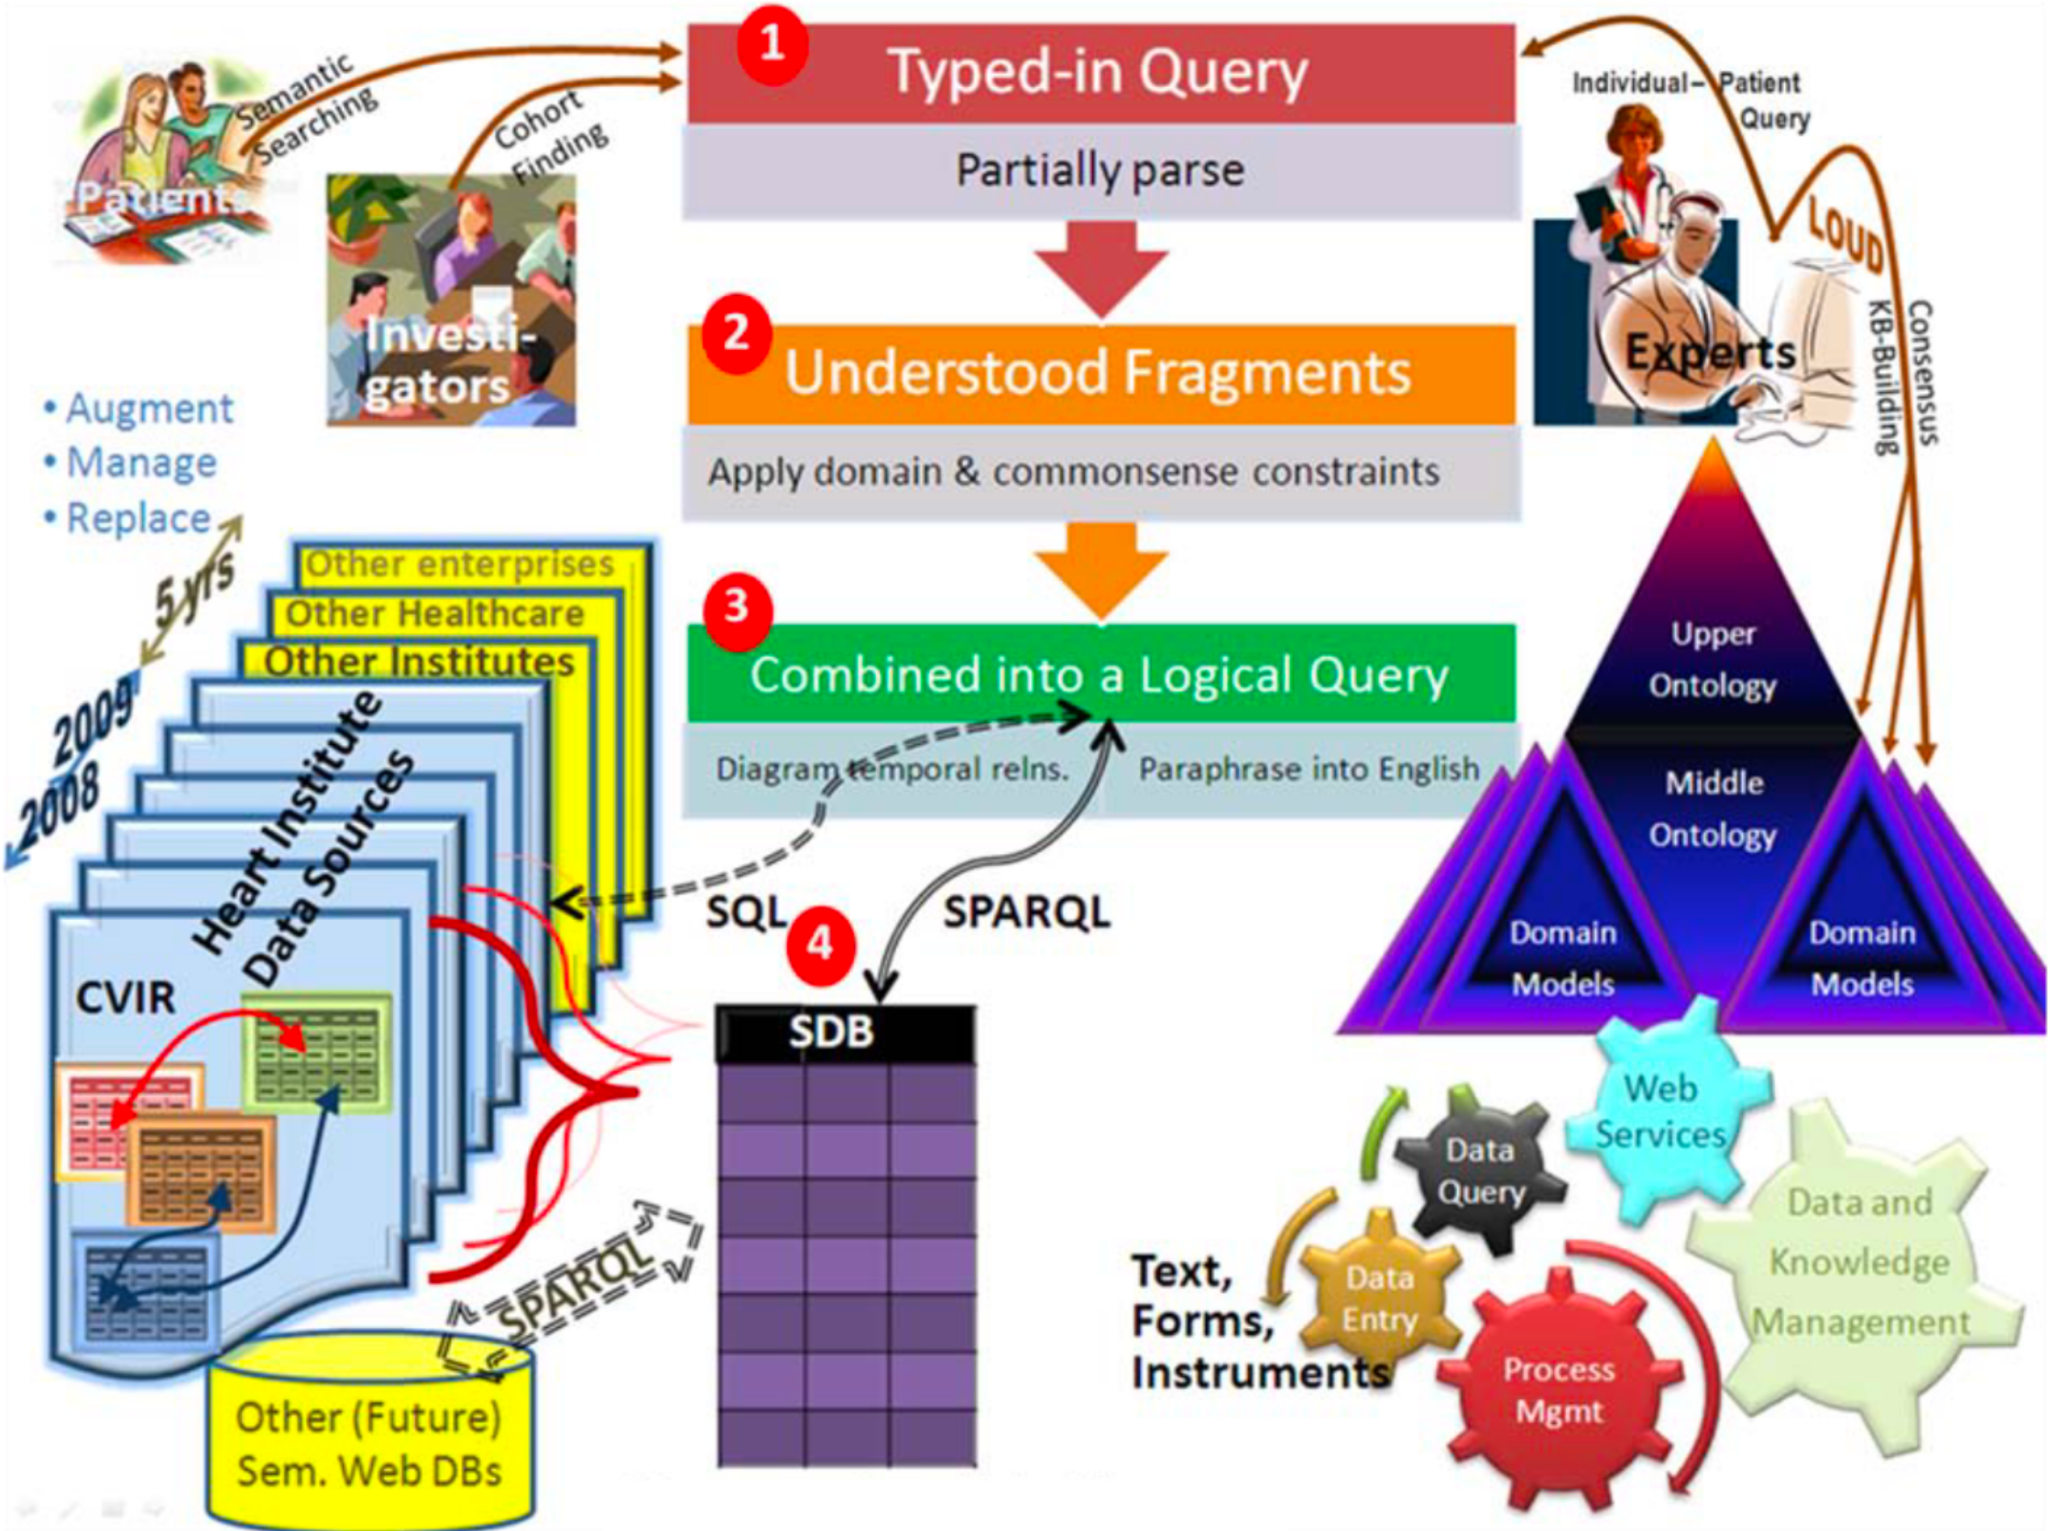
\includegraphics[width=\linewidth]{figures/f13.png}
        \caption[The Semantic Research Assistant (SRA) query-handling workflow]{\textbf{The Semantic Research Assistant (SRA) query-handling workflow} \citep[p. 7]{lenat_harnessing_2010}. Used with permission.}
        \label{fig:13}
    \end{minipage}%
    \hfill
    \begin{minipage}[t]{0.48\linewidth}
        \centering
        \includegraphics[width=\linewidth]{figures/f13r.png}
        \caption[Detail based on the Lenat et al. SRA query-handling workflow]
        {\textbf{Detail based on the Lenat et al. SRA query-handling workflow} \citep[p. 7]{lenat_harnessing_2010}.}
        \label{fig:14}
    \end{minipage}
\end{figure}
\FloatBarrier
\index[terms]{Cone Semantic Form} 


\subsection{Knowledge Translation}
I borrow the term Knowledge Translation (KT) from healthcare as a term that can be used within information as a whole, in sustainability or otherwise. In 2009, the Canadian Institutes of Health Research (CIHR) defined KT as “a dynamic and iterative process that includes the synthesis, dissemination, exchange and ethically sound application of knowledge to improve health, provide more effective health services and products and strengthen the healthcare system” \citep[p. 4]{straus_knowledge_2009-1}. 
\index[terms]{Knowledge Translation (KT)}

Climate crisis mitigation is facing overlapping challenges with health care systems when it comes to information management. In Knowledge Translation in Healthcare (2009), Straus and Tetroe report that healthcare systems are “faced with the challenge of improving the quality of care and decreasing the risk of adverse events” \citep[p. 3]{straus_knowledge_2009-1}. “Globally, health systems fail to optimally use evidence, resulting in inefficiencies and reduced quantity and quality of life” \citep[p. 3]{straus_knowledge_2009-1}. The “science and practice” of KT can help answer these challenges \citep[p. 3]{straus_knowledge_2009-1}. Similarly to the mission that drives KA in the climate crisis, closing knowledge-to-action gaps drives KT because providing evidence from research is “necessary but not sufficient for providing optimal care delivery” \citep[p. 3]{straus_knowledge_2009-1}. We might even take on the characteristics of care used in KT to further elevate the quality of human relationships we want to foster in all climate resilience KA. Knowledge Production, “distillation, and dissemination are not sufficient on their own to ensure implementation in decision making” in the “move beyond simple dissemination of knowledge to actual use of knowledge” \citep[p. 4]{straus_knowledge_2009-1}. This insufficiency is also present in climate crisis mitigation outcomes in a Sustainability Transitions Knowledge Activation (STKA).
\index[terms]{Knowledge Activation (KA)} 
\index[terms]{Knowledge Translation (KT)}
\index[terms]{Knowledge Production (KP)}
\index[terms]{climate resilience}

\subsubsection{Interdisciplinary visual methods}
\label{Interdisciplinary visual methods}

Symbolic representations of information facilitate the analysis between knowledge domains. For example, Goethe’s studies of morphology are activated into practice by Gemma Anderson-Tempini’s work. Anderson-Tempini “presents drawing as a means of developing and disseminating knowledge, and of understanding and engaging with the diversity of natural and theoretical forms, such as animal, vegetable, mineral, and four-dimensional shapes” \citep[back cover]{anderson_drawing_2018}.
\index[people]{Goethe, Johann Wolfgang von}

Anderson-Tempini defines isomorphology as “an alternative approach to classification through drawing” that “adapts Goethe’s morphological approach” \footnote{For a thorough discussion of Goethe's morphological approach see \textit{Morphology: Questions on Method and Language} \citep{molder_morphology_2013}.} to “the study of form and symmetry in whole organisms towards a focus on the parts of organisms” which “initiates a move from observation to abstraction” \citep[p. 11]{anderson_drawing_2018} \footnote{For an illustration of Anderson-Tempini’s isomorphologies see her illustration \textit{Fig 1: The primary forms and symmetries of Isomorphology} \citep{anderson_what_2013}.}. She proposes a set of “conceptual forms [...] abstracted from nature”. Specifically, she proposes thirteen “primary forms and symmetries of isomorphology” \citep{anderson_what_2013}.
\index[people]{Anderson-Tempini, Gemma}
\index[people]{Goethe, Johann Wolfgang von}
\index[terms]{isomorphology}

Anderson-Tempini’s isomorphological drawing practice is also used to represent the change over time of a given subject, ``representing morphology as a dynamic and formative process” \citep[p. 179]{anderson_drawing_2018}. This practice, called isomorphogenesis ``progresses from the empirical study of the morphology of static museum specimens towards a conceptual study that aims to draw morphology as dynamic” \citep[p. 179]{anderson_drawing_2018}. Isomorphogenesis is a ``drawing practice or `experiment'" \citep[p. 179]{anderson_drawing_2018} that captures ``four-dimensional shapes” \citep[back cover]{anderson_drawing_2018} to explore the ``potentialities of representing morphology as a dynamic and formative process”  \citep[p. 179]{anderson_drawing_2018}. Isomorphogenesis ``progresses from the empirical study of the morphology of static museum specimens towards a conceptual study that aims to draw morphology as dynamic” \citep[p. 179]{anderson_drawing_2018} \footnote{For an example of isomorphogenesis see ``Figure 15: `Isomorphogenesis’ no.10” \citep[p. 203]{anderson_drawing_2018}.}. In short, isomorphogenesis as a drawing practice illustrates the dynamic changes of a given organism over time facilitating their deeper study.
\index[people]{Anderson-Tempini, Gemma}

The impact of Anderson-Tempini’s isomorphology and isomorphogenesis practice extends internationally. This approach is formally recognized and ``has developed as a visual counterpart for the European Research Council-funded project `A process ontology for biology’, led by Professor John Dupré at the University of Exeter” \citep[p. 179]{anderson_drawing_2018}. Anderson-Tempini’s isomorphology and isomorphogenesis methods contribute substantially to classifying natural forms and visualizing their dynamic traits and transformations through drawing.
\index[people]{Anderson-Tempini, Gemma}
\index[terms]{isomorphology}

\subsection{Knowledge Production}
To recap, KSSTP stands for Knowledge Surfacing, Synthesis, Translation, and Production. This section, Knowledge Production, concludes the literature review section dedicated to defining the terms and dynamics involved in KSSTP.
\subsubsection{Induction, deduction, and abduction in Peirce}
Within KSSTP, Sowa’s understanding of Peircean analogy is closer to what I mean by Knowledge Surfacing; Adler’s ``syntopical reading” and Wilson’s consilience are closer to what I mean by Knowledge Synthesis. Peircean abduction is closer to what I mean by Knowledge Production because it is about proposing something new. In fact, Peirce defines abduction as ``the process of forming an explanatory hypothesis”, the “only logical operation which introduces any new idea”, and the only means to ``learn anything or to understand phenomena at all"  \citep[p. 106]{peirce_pragmatism_1960}. 
\index[terms]{abduction}
\index[people]{Peirce, Charles Sanders}
\index[people]{Sowa, John F.}
\index[people]{Adler, Mortimer J.}
\index[people]{Wilson, Edward O.}
\index[terms]{syntopical reading}
\index[terms]{Knowledge Surfacing (KSu)}
\index[terms]{Knowledge Synthesis (KSy)}
\index[terms]{Knowledge Production (KP)}
\index[terms]{consilience}
\index[terms]{analogy} 

Peirce elaborates that induction ``does nothing but determine a value"  and ``shows that something actually is operative"; deduction ``merely evolves the necessary consequences of a pure hypothesis" and ``proves that something must be"; abduction ``merely suggests that something may be", and ``Its only justification is that from its suggestion deduction can draw a prediction which can be tested by induction" \citep[p. 106]{peirce_pragmatism_1960}. In the case of the title of this thesis, it is the \textit{may} in the \textit{What may be known}. 
\index[people]{Peirce, Charles Sanders}
\index[terms]{abduction}


The mystery of introducing ``any new idea” \citep[p. 106]{peirce_pragmatism_1960} is captured by Peirce when he wrote: ``No reason whatsoever can be given for it, as far as I can discover; and it needs no reason, since it merely offers suggestions” \citep[p. 106]{peirce_pragmatism_1960}. It would seem that curiously that the illusive Knowledge Production is vital to moving any theory forward, and yet its abduction ``needs no reason” and constitutes only a proposal for the direction of further study, relying on the other forms of logical operation to constitute if it ``may be” or ``must be” \citep[p. 106]{peirce_pragmatism_1960}.
\index[people]{Peirce, Charles Sanders}
\index[terms]{abduction}
\index[terms]{Knowledge Production (KP)}


Wilson’s borderland disciplines \citep[p. 12]{wilson_consilience_1999} and Adler’s \textit{Syntopicon} can work together in syntopical consilience as a means towards creating ``new language” \citep[p. 185]{pangaro_design_2011}. Syntopical consilience offers the possibility of Peircean abduction or introducing a ``new idea” \citep[p. 106]{peirce_collected_1960}. Therefore, I propose that in KSSTP, the confluence of Knowledge Synthesis, Knowledge Translation, and Knowledge Production can be referred to as Syntopical Consilient Abduction.
\index[terms]{abduction}
\index[people]{Pangaro, Paul} 
\index[people]{Peirce, Charles Sanders}
\index[people]{Adler, Mortimer J.}
\index[terms]{Syntopicon}
\index[terms]{Knowledge Translation (KT)}
\index[terms]{Knowledge Production (KP)}
\index[terms]{consilience}
\index[terms]{syntopical consilience}


\section{Design across KSSTP}
\noindent Design works across the various forms of KSSTP, surfacing, synthesizing, translating, and creating: surfacing by revealing relationships between ideas in techniques like topic modelling, synthesizing by combining ideas in techniques like Systematic Combining \citep[p. 554]{dubois_systematic_2002}, translating by framing ideas from one discipline in the ways that another can receive and understand \citep[p. 3]{straus_knowledge_2009-1} and creating in generative methods like gigamapping \citep{sevaldson_giga-mapping_2011}. In this section, we will cover various forms of design that relate to KSSTP within discussions of composition, spatial composition, visual forms of Knowledge Production, information design, Systems Oriented Design, Systematic Combining, Design for Sustainability Transitions, and the torus as an isomorph for visual reasoning.
\index[people]{Sevaldson, Birger} 
\index[terms]{gigamapping}
\index[terms]{Systematic Combining (SC)}
\index[people]{Gadde, Lars-Erik}
\index[people]{Dubois, Anna}
\index[terms]{torus}
\index[terms]{Knowledge Surfacing (KSu)}
\index[terms]{Knowledge Production (KP)}
\index[terms]{Systems Oriented Design (SOD)}

To ``distinguish design from Design”, Sevaldson notes that B. Archer “made a distinction between design and Design with a capital D [...]. Design with a Capital D is a third area of knowledge and education equal to science and the humanities, with relations to arts and technology” \citep[p. 91]{sevaldson_designing_2022}. In Archer’s own words: ``Design, in its most general educational sense, where it is equated with Science and the Humanities, is defined as the area of human experience, skill and understanding that reflects man’s concern with the appreciation and adaptation of his surroundings in the light of his material and spiritual needs. In particular, though not exclusively, it relates with the configuration, composition, meaning, value and purpose in man-made phenomena” \citep[p. 20]{archer_design_1979}. Archer, as cited by Sevaldson, thus posits Design as a distinct knowledge domain alongside science and the humanities.
\index[people]{Sevaldson, Birger}

Sevaldson entreats: ``It is urgent to develop and reinforce this perspective of Design as an equal area to science and the humanities. Design should be viewed as a unique mode of knowledge production that can be used to achieve the systemic changes needed for future systemic innovations” \citep[p. 91]{sevaldson_designing_2022}. Furthermore, Sevaldson articulates: ``Design is inherently systemic. Any design must relate to users, production methods, culture, aesthetics, business economy, and technology. In that sense, it is always a result of negotiation and navigation within networks of relations between large complex systems. Without putting in the effort to understand, to the best of our abilities, these networks of relations, one will not be able to produce design outs that function well in the world” \citep[p. 91]{sevaldson_designing_2022}. Sevaldson posits Design as a systemic knowledge domain crucial for innovation and navigating complex interdisciplinary relational networks.
\index[people]{Sevaldson, Birger}
\index[terms]{Knowledge Production (KP)}

Epistemologically, I posit that Archer's Design, as opposed to lowercase-d design, is a semantic field for Wilson's consilience, in which it is possible to further integrate Science and the Humanities.
\index[people]{Wilson, Edward O.}
\index[terms]{consilience}


\subsection{Composition}
To define the composition, we must first consider what it means to be `whole.’ At first glance, the famous aphorism ``The whole is greater than the sum of the parts” captures the core of Gestalt psychology. This statement is often attributed to Aristotle, or to Systems Thinking \citep[p. 164]{sevaldson_designing_2022}\footnote{For a more fulsome retracing of the lineage of thinkers that lead to Systems Thinking as a practice, see ``History and State of Systems Thinking in Design” in Sevaldson (2022), p. 149-150 \citep[p. 148-150]{sevaldson_designing_2022}.}, but it merits clarification. To cite Gestalt psychologist Kurt Koffka in Sevaldson, ``The whole is other than the sum of its parts” \citep[p. 164]{sevaldson_designing_2022}\footnote{For a more fulsome connection between Gestalt and design and systems see ``Gestalt Psychology” in Sevaldson (2022), p. 186-188 \citep[p. 163-167]{sevaldson_designing_2022}.}. Koffka’s statement is closer to the words of Aristotle, who wrote ``the whole is something beside the parts” \citep{aristotle_metaphysics_1989}. To treat with composition, we need to recognize the ways wholes have properties distinct from their parts' properties.
\index[people]{Sevaldson, Birger}

Composition, or the interpretation of wholes and parts, is fundamental to understanding. Noam Chomsky argues that composition is foundational to language \citep{chomsky_knowledge_1986,chomsky_syntactic_2002}, Sevaldson suggests that it is ``the most important notion of design” \citep[p. 162]{sevaldson_designing_2022}, and Geman et al. argue it is “fundamental to all of cognition” \citep[p. 1]{geman_composition_2002}. Furthermore, Geman et al. define composition the semantics engaged in composition as the ability ``to represent entities as hierarchies of parts, with these parts themselves being meaningful entities, and being reusable in a near-infinite assortment of meaningful combinations” \citep[p. 1]{geman_composition_2002}. As Sevaldson puts it: ``Composition in design can be understood as a special way of synthesis in shape and form. In art, composition rests on its own objective, and creates its own logic” \citep[p. 167]{sevaldson_designing_2022}. Composition (i.e., the way we combine and interpret parts to create a whole) is fundamental to understanding language, design, and cognition.
\index[people]{Sevaldson, Birger}
\index[terms]{composition}

In the converse of \textit{composition}, Sevaldson offers additional subtlety to the discussion of \textit{decomposition}. Sevaldson writes object-oriented approaches offer less emphasis on the relation between entities, which ``comes as a natural consequence of their reference to language, where the relation between the words (entities) is proximal rather than a potential process or signal by its own right” \citep[p. 169]{sevaldson_designing_2022}. In this thesis, I adopt an approach closer to Sevaldson’s, where the relation between entities in composition is itself a signal that carries its own meaning.
\index[people]{Sevaldson, Birger}
\index[terms]{composition}


\subsection{Spatial composition}
Further to visual experience in space, treatments of spatial composition exist. In Semiotics of \textit{visual language} (1990), Saint-Martin introduces a syntax of sculptural language and its laws, including topological relations, by using the infrastructure of the virtual cube as corresponding ``to the contour of the most unified geometrical forms”, and having ``preeminent status in the perceptual process” \citep[p. 173-174]{saint-martin_semiotics_1990}. Proposing to work within the gestaltian cube continues to be a distinctly Euclidean perspective. While I appreciate that the constraints of point-plotting within the cube can provide a starting point, other methods of plotting points and examining their relationships exist, such as the embedding into spherical space, hyperbolic space, and custom metric space \citep{mcinnes_embedding_2018}.
\index[people]{Saint-Martin, Fernande}
\index[terms]{composition}

Saint-Martin, however, goes on to distinguish the types of mathematics used to understand meaning-making in three-dimensional space. She recalls that in ``the 1940s, the genetic epistemology of Piaget established that the first geometrical model of space used by human beings is not Euclidian geometry but topology. This spatial model of the organization of perceptual experience remains throughout human life the basic means by which one constructs his notions of reality” \citep[p. 68]{saint-martin_semiotics_1990}. 
\index[people]{Saint-Martin, Fernande}
\index[terms]{topology}

Saint-Martin and Johanna Drucker, author of \textit{Graphesis} (2014), imagine futures with integration of topological semantic expression. In The Semiotics of Visual Language Saint-Martin writes that she is ``entrusting to a future work the development of the semantic system of topological semiotics” \citep[p. 225]{saint-martin_semiotics_1990}  Drucker proposes that topological concepts could be useful in analyzing “textual structures” and ``paratextual apparatuses”, including marginal notes, footnotes, and layout features \citep[p. 54]{drucker_graphesis_2014}. She emphasizes that understanding continuity and discontinuity in text interpretation is crucial for interpreting hyperlinked environments \citep[p. 54]{drucker_graphesis_2014}. However, Drucker notes that we still need to develop a specialized `metalanguage’ to describe how graphical elements convey relationships in digital spaces and how they contribute to the text's meaning through their ``structuring effects” \citep[p. 54]{drucker_graphesis_2014}. Drucker poignantly muses with the imagery of space: ``Thought forms expressed in the constellationary field may be abstracted and studied for their configuration of knowledge as well as their content, and the organizing orders of graphical expression will take on their own legibility” \citep[p. 196]{drucker_graphesis_2014}. Saint-Martin and Drucker envision a future where topological concepts are integrated into semantic and textual analysis, emphasizing the need for a new language to interpret graphical relationships in digital spaces.
\subsection{Visual Forms of Knowledge Production}
Johanna Drucker might categorize the diagrams which Tversky sees as a ``platform for inference” as ``visual forms of knowledge production” \citep{drucker_graphesis_2014} distinct from visual forms of information display. In fact, Drucker defines graphesis as ``the study of the visual production of knowledge” \citep[p. 3]{drucker_graphesis_2014}.
\index[people]{Drucker, Johanna}
\index[people]{Tversky, Barbara}
\index[people]{Saint-Martin, Fernande}

More widely than diagrams and interface, Drucker’s work offers much-needed clarity in visual epistemology, or ``ways of knowing that are presented and processed visually” \citep[p. 8]{drucker_graphesis_2014}. She underscores the epistemological urgency of this thesis when she writes: ``Visual expressions of knowledge are integral to many disciplines in the natural sciences, but language-oriented humanities traditions have only barely engaged with visual forms of knowledge” \citep[p. 7]{drucker_graphesis_2014}. Drucker’s insights in visual epistemology extend beyond diagrams and interfaces to include \textit{visual arguments}. Tversky found that when it comes to visual arguments and visual reasoning as a whole, ``well-crafted diagrams are superior to language for explaining many kinds of information—more directly, more succinctly” \citep{tversky_barbara_2022}. Furthermore, visual explanations are ``a check for coherence, a check for completeness, and a platform for inference” \citep{tversky_barbara_2022}. In other words, well-made graphs are worth more than a thousand words, specifically because they can act as visual arguments and help us reason through complex information in ways that are more effective than using only words. 
\index[people]{Drucker, Johanna}
\index[people]{Tversky, Barbara}

Drucker argues that information visualizations often present themselves as objective representations of data when, in fact, they are interpretative arguments made through visual means \citep[p. 10]{drucker_graphesis_2014}. Drucker points out the paradox of how visual forms of knowledge production across various media tend to conceal the visual ways arguments get constructed \citep[p. 10]{drucker_graphesis_2014}. Drucker’s book aims to highlight these visual forms of knowledge production and develop a critical framework for analyzing them. 
\index[people]{Drucker, Johanna}

\subsubsection{Graphical User Interface (GUI)}
%\noindent \textbf{GUI} \\
In a historical context when ``we carry on most of our personal and professional business through interfaces”, it is pertinent to single out that ``no single innovation has transformed communication as radically in the last half century as the GUI”, the Graphical User Interface \citep[p. 8]{drucker_graphesis_2014}. The importance of the GUI is in no small part because of its graphesis. 
\index[people]{Drucker, Johanna}

Drucker encouragingly describes the simultaneously technical and interpretative endeavour of graphesis as a view ``into the studio laboratory of knowledge design, where we sit at the consoles of workstations meant to help engineer and imagine the creation and implementation of a diagrammatic and constellationary rhetoric, of writing in the infinitely extensible field populated by new conventions of legibility that structure and organize expression and communication” \citep[p. 197]{drucker_graphesis_2014}. Drucker then adds that ``the workstation dissolves into infinite play of text and task, knowledge as performance and invention, a cognitive engine engaged with the collective life of embodied mind” \citep[p. 197]{drucker_graphesis_2014}. Drucker’s description of the studio laboratory of knowledge design is a more humanistic facet of the more computer-science-oriented approach called knowledge engineering, or the use and construction of a computational knowledge-based system used for problem-solving \citep[p. 8]{wielinga_kads_1992}. Drucker’s sense of graphesis as a technical and interpretative endeavour sets the stage for a more humanistic approach to knowledge design.
\index[people]{Drucker, Johanna}
%``Cognitive engine" \citep[p. 197]{drucker_graphesis_2014}.
 
The ``subjective display of humanistic phenomena can be applied across” domains in the following ``four basic levels” of ``visualizing interpretation” \citep[p. 135]{ drucker_graphesis_2014} or ``visual forms knowledge production” \citep{drucker_graphesis_2014}: 
“1) Modeling phenomenological experience in the making of humanities (\textit{data} as \textit{capta}, primary modeling, the representation of temporal and spatial experience); 
2) Modeling relations among humanities documents, i.e., discourse fields (a different metric might be needed to understand dates on diplomatic documents from the spring of 1944 or 1950); 
3) Modeling the representations of temporality and spatiality that are found in humanities documents (narrative is the most obvious); 
4) Modeling the interpretation of any of the above (depicting or graphing the performative quality of interpretation)” \citep[p. 135]{ drucker_graphesis_2014}. 
\index[people]{Drucker, Johanna}
\index[terms]{capta}

\subsubsection{Humanistic Design}
The ``humanist commitment to interpretation”, ``embracing ambiguity […,] contradictions and the lack of fixity or singularity”, and the ways that “forms of classification, taxonomy, or information organization embody ideology” \citep[p. 178]{drucker_graphesis_2014} are not mutually exclusive to the value of synthesis across ideology and taxonomy. Wilson’s borderland disciplines and Adler’s \textit{Syntopicon} are evidence of how ambiguity can coexist and even benefit from the synthetic “fixity” (i.e., artificial stability) of consilience and syntopical reading, ideological or otherwise. In fact, Drucker later revisits this comingling of “fixity” and ambiguity in the afterword of \textit{Graphesis}: “The interpretative and the empirical need not exclude each other. So the graphic grammar of an emerging visual system inclined to present the embodied, situated, circumstantial, and fragmentary quality of knowledge will embrace specificities and particularities even as it makes possible the social mediation of communicative exchange” \citep[p. 196]{drucker_graphesis_2014}.
\index[people]{Drucker, Johanna}
\index[people]{Adler, Mortimer J.}
\index[people]{Wilson, Edward O.}
\index[terms]{Syntopicon}
\index[terms]{syntopical reading}
\index[terms]{consilience}

Drucker’s \textit{Graphesis} captures an ontological ethos for humanistic information design in which she advocates for advancing beyond the terms “set by disciplines whose fundamental beliefs are antithetical to interpretation” \citep[p. 178]{drucker_graphesis_2014}. In her vision of critical design for interpretative and humanistic interfaces, Drucker emphasizes the importance of revealing the constructedness of knowledge and facilitating interpretative activity with tolerance for “inconsistency among types of knowledge representation, classification, fluid ontologies, and navigation” \citep[p. 178]{drucker_graphesis_2014}. Drucker’s work lays the foundation for the evolution of scholarly tools toward more dynamic, relational, and interpretative approaches in humanistic information design.
\index[people]{Drucker, Johanna}

Drucker argues that we “are in the incunabula of information design” \citep[p. 176]{drucker_graphesis_2014}. She identifies emerging “new conventions that do not rely on book structures” \citep[p. 176]{drucker_graphesis_2014} in information software. Drucker emphasizes that the “new condition for scholarly activity is relational and dynamic”, prioritizing process over product \citep[p. 176]{drucker_graphesis_2014}. She notes that ``Informational derivatives of data mining, analytics, visualization, and display are increasingly a part of a reading environment in scholarly, political, and business activity” to visualize “these networked relations, communities of scholarly exchange, argument, comment, linked references, framings, and embedded citations” \citep[p. 176]{drucker_graphesis_2014}. Drucker advocates for “an interface that is meant to expose and support the activity of interpretation, rather than to display finished forms” \citep[p. 179]{drucker_graphesis_2014}, representing a shift towards praxis in humanistic information design. Drucker envisions the dawn of humanistic information design as emphasizing dynamic and interpretative interfaces that visualize networked scholarly discourse and prioritize process over finished products.
\subsection{Information visualization and information design }
Drucker defines information graphics and information visualization as “visualizations based on abstractions of statistical data”, or “metrics expressed as graphics” \citep[p. 7]{drucker_graphesis_2014}. Sevaldson writes that information visualizations make information “accessible and understandable” \citep[p. 186]{sevaldson_designing_2022}. The impact of information visualization has been great, ``and in many cases, the visual serves as scientific (ostensive) proof” \citep[p. 186]{sevaldson_designing_2022}. Information visualization is a valuable practice for displaying the various modes of Knowledge Activation. 
\index[people]{Drucker, Johanna}

Data “does not have an inherent visual form”, so visualizations are also necessarily interpretations \citep[p. 7]{drucker_graphesis_2014}. Information visualization “creates a bridge between sciences and the arts. It is often aesthetic decisions that influence the interpretation of the visualisations” \citep[p. 186]{sevaldson_designing_2022}. The interpretativeness of information visualizations, and data representations more generally, are a means of bridging art and science through aesthetic decisions that shape them.
\index[people]{Drucker, Johanna}

However, the limitation of information visualization is that it is “with very few exemptions, descriptive”, and often this happens through “simplification and reduction of the complexity of the material” \citep[p. 186]{sevaldson_designing_2022}.
\index[people]{Sevaldson, Birger}


\subsection{Systems Oriented Design (SOD)}
The complexity of science and design research as a field of Knowledge Production ``demands an equally rich repertoire of interrelated methods and positions” \citep[p. 8]{sevaldson_discussions_2010-1}. 
\index[people]{Sevaldson, Birger}
\index[terms]{Knowledge Production (KP)}
\index[terms]{Systems Oriented Design (SOD)}

As introduced earlier, one such codified repertoire is Systems-Oriented Design (SOD), an interdisciplinary methodology that combines systems thinking with design practice to tackle super-complex multi-level problems by integrating diverse information in generative rather than descriptive means \citep[p. 27, p. 152, p. 157]{sevaldson_designing_2022}. SOD is a “dialect” in the larger field called Systemic Design which is distinguished by its inclination towards design practice. SOD is also sometimes called the Oslo-School of Systemic Design \citep[p. 2]{sevaldson_designing_2022}\footnote{For a more fulsome retracing of how Systemic Design emerged as a field see “Systemic Design: The Renaissance of Systems Thinking in Design” \citep[p. 186-188]{sevaldson_designing_2022}.}.
\index[terms]{Systemic Design}
\index[people]{Sevaldson, Birger}

Central to SOD is the practice of gigamapping, a technique for visually representing complex systems and their interconnections \citep[p. 26]{sevaldson_designing_2022}. Notably, gigamapping avoids hierarchy and orients practitioners to investigate relationships and meta-relationships like unknown unknowns \citep[p. 55, p. 353-357]{sevaldson_designing_2022}. These principles speak to the utility of gigampping as a post-structuralist tool for the definition of systems and ideas. SOD integrates constructivist learning in a way that emphasizes the designer's role in shaping systems through continuous exploration, intervention, and adaptation \citep[p. 153]{sevaldson_designing_2022} \footnote{For a retracing of constructivist learning theory, Sevaldson notes that it has been influenced by Lev Vygotsky, Herbert Simon, Heinz von Foerster, and Humberto Maturana \citep[p. 153]{sevaldson_designing_2022}.}
\index[people]{Sevaldson, Birger}
\index[terms]{gigamapping}

In Sevaldson, we find an example of how the network graph provides a distinctly useful medium for managing the discussed epistemological ambiguity in a versatile, decentralized, interdisciplinary representation of entities and relationships, namely, Christopher Warnow's \textit{Map of Systems Theory} (2012) \citetext{\citealp[p. 125]{sevaldson_designing_2022}; \citealp{warnow_map_2012}}. 
\index[people]{Sevaldson, Birger}

Systems Oriented Design encourages systemic designers to understand the dynamics of systems and intervene at various levels while considering the ethics, ripple effects, and consequences of their work \citep[p. 95-96]{sevaldson_designing_2022}. This includes “evaluating and re-evaluating the constructed boundary when working with a system” \citep[p. 146]{sevaldson_designing_2022}, or boundary critique \citep{midgley_theory_1998}.
\index[terms]{Systemic Design}
\index[people]{Sevaldson, Birger}
\index[terms]{Systems Oriented Design (SOD)}

Here at OCAD University, Peter Jones compiled the practice of synthesis mapping based on Sevaldson’s gigamap method \citep[p. 129]{jones_synthesis_2017} in and through the Strategic Innovation Lab (sLab). Jones, Shakdher and Singh used the synthesis map method in the Knowledge Translation of Healthcare Systems \citep[p. 129]{jones_synthesis_2017}. 
\index[terms]{gigamapping}
\index[terms]{Knowledge Translation (KT)}
 \clearpage

 \FloatBarrier
\begin{figure}[h]
    \centering
    \includegraphics[width=0.6\linewidth]{figures/f15.png}
    \caption[Diagram of the SOD Creative Process Framework]
    {\textbf{Diagram of the SOD Creative Process Framework} \citep[p. 312]{sevaldson_designing_2022}. Used with Sevaldson's permission.}
    \label{fig:15}
\end{figure}

\begin{figure}[h]
    \centering
    \includegraphics[width=0.6\linewidth]{figures/f18.png}
    \caption[Diagram of a design process with iterations]{\textbf{Diagram of a design process with iterations} \citetext{\citealp[p. 343]{sevaldson_designing_2022}; \citealp{sevaldson_designing_2022-1}}. Used with Sevaldson's permission.}
    \label{fig:18}
\end{figure}
\FloatBarrier

\FloatBarrier
\begin{figure}[h]
    \centering
    \includegraphics[width=0.6\linewidth]{figures/f16.png}
    \caption[An example gigamap]
    {\textbf{An example gigamap}. Making Waves: Organizational gigamap by Angel L. Lamar Oliveras \citep{lamar_oliveras_making_2020}. Used with permission under the CC-BY-NC-ND 4.0 International License.}
    \label{fig:16}
\end{figure}
\index[terms]{gigamapping}

\begin{figure}[h]
    \centering
    \includegraphics[width=0.6\linewidth]{figures/f17.png}
    \caption[Key to example gigamap]
    { \textbf{Key to example gigamap} \citep{lamar_oliveras_making_2020}. 
Used with permission under the CC-BY-NC-ND 4.0 International License.}
    \label{fig:17}
\end{figure}
\FloatBarrier

\subsection{Systematic Combining (SC)}
If climate is everyone’s problem, and climate is a system of systems, then systems approaches are everyone’s problem, including designers. Robust Systemic Design approaches to sustainability are emerging, like the recent work of Svein Gunnar Kjøde, a student of Birger Sevaldson.
\index[terms]{Systemic Design} 
\index[terms]{Systematic Combining (SC)}

The systems approach to research called Systematic Combining (SC) is the central strategy for Kjøde’s Entanglement of Systemic Design and Sustainability Transitions (2024). Dubois and Gadde proposed the term “systematic combining” in 2002 and described it as “a process where theoretical framework, empirical fieldwork, and case analysis evolve simultaneously, and it is particularly useful for development of new theories” \citep[p. 554]{dubois_systematic_2002}. They note that the “main characteristic of this approach is a continuous movement between an empirical world and a model world” \citep[p. 554]{dubois_systematic_2002} “grounded in an ‘abductive’ logic” \citep[p. 553]{dubois_systematic_2002}. Systematic Combining offers a dynamic approach to theory development through the simultaneous evolution of framework, fieldwork, and analysis. The application of SC in sustainability transitions research highlights its ability to handle complex, interconnected, and emergent phenomena.
\index[terms]{abduction}
\index[terms]{Systemic Design}
\index[terms]{Systematic Combining (SC)}
\index[people]{Gadde, Lars-Erik}
\index[people]{Dubois, Anna}


Systematic combining de-emphasizes data verification and accuracy. Instead, it leverages how “multiple sources may contribute to revealing aspects unknown to the researcher, i.e., to discover new dimensions of the research problem” \citep[p. 556]{dubois_systematic_2002}. “As such,” Kjøde explains, “the approach arguably supports an investigation that navigates rapidly developing, interdisciplinary fields of knowledge that not only study the systemic phenomena of sustainability transitions but becomes a system of dynamic knowledge in itself” \citep[p. 46]{kjode_entanglement_2024}. According to Sevaldson and Kjøde, systems-oriented design inquiry methods must be able to handle interrelation and contradiction of ideas \citetext{\citealp[p. 46]{kjode_entanglement_2024}; \citealp[p. 8]{sevaldson_discussions_2010-1}}. Kjøde writes that his choice to use SC in his doctoral work “responds directly to the complex, interconnected and emergent nature of the sustainability transitions field” \citep[p. 45]{kjode_entanglement_2024}. Systematic Combining prioritizes discovering new research dimensions through multiple sources, making it well-suited for complex interdisciplinary fields like climate crisis KA, which requires handling interrelated, evolving, and contradictory ideas.
\index[people]{Kjøde, Svein Gunnar}
\index[terms]{Systematic Combining (SC)}
\index[people]{Gadde, Lars-Erik}
\index[people]{Dubois, Anna}


\subsection{Design for Sustainability Transitions (DfST)}
 Grin et al. define Sustainability Transitions (ST) as “radical transformation towards a sustainable society” \citep[p. 1]{grin_introduction_2011} involving an axiological “quest for new value systems” \citep[p. 2]{grin_introduction_2011}, “a shift to a more sustainable economy” \citep[p. 1]{grin_introduction_2011}, and “long-term and complex socio-technical transitions” \citep[p. 11]{geels_introduction_2011}. Design for Sustainability Transitions (DfST), also called Transition Design, is a “kind of designing that is connected to long horizons of time and visions of sustainable futures” \citep[p. 3]{irwin_transition_2015}. In short, sustainability-oriented multi-systemic interdisciplinary information processes and their societal outcomes are supported by Design for Sustainability Transitions. 

Flittner et al. (2022) elaborate that DfST combines frameworks and methods from a variety of fields, like transition management, anthropology, design research, and sustainability science, towards a practice for building enduring “transitions towards more sustainable societies” \citep[p. 160]{flittner_design_2022}. ST and DfST are both, then, interdisciplinary, longitudinal, iterative, multi-praxis, multi-systemic, cross-sectoral theoretical work which sustains the potential for “complementary understandings” \citep[p. 197]{oztekin_co-positioning_2020} and operationalization of social change. Furthermore, DfST engages three embedded levels of Systemic Design complexity described by Robert Young: (a) ``design in context" or ``design at the level of products and artefacts”, (b) ``designing context” or ``design at the level of systems and services”, and (c) ``design of context” or ``design at the level of policy, ideology, purposes, values and norms” \citep[p. 200]{oztekin_co-positioning_2020}.

All design must take into account ST, and in some sense, all responsible design is DfST. As such, this thesis works towards ST through KA, or STKA for short.
\index[terms]{Systemic Design}

\subsection{The torus}

\subsubsection{Torus isomorph as a composition for visual reasoning}
The torus, with its captivating visual and mathematical properties, emerges as an isomorph in diverse disciplines and contexts. My initial encounter with the torus was through interpretations of chakra geometry whereby tori are used to represent cyclical energy fields in and around the human body \citep{singer_quantum_2019}.
\index[terms]{torus}
\index[terms]{composition}

In \textit{Rudy Rucker's Infinity and the Mind (2005)}, the torus is employed to model space-time, depicting an oscillating universe with circular time. Rucker's toroidal model suggests a universe where time loops back onto itself in a continuous cycle as shown in \autoref{fig:19}. In 2013, the Resonance Science Foundation (RSF) produced an animation of the yin yang mapped onto a torus. This work is an example of how paradoxes of the cosmological imagination can be visuospatialized using the torus
\citep{resonance_science_foundation_yin_2013}.

\index[people]{Rucker, Rudy}
\index[terms]{torus}

As I directed my research away from cosmology in this thesis, I continued to encounter the torus in a surprising variety of fields in ways that captured a variety of phenomena. For example, Gardner et al. use TDA of the recordings of hundreds of rat grid cells to demonstrate that ``the joint activity of grid cells from an individual module resides on a toroidal manifold" \citep[p. 123]{gardner_toroidal_2022}, as shown in \autoref{fig:20}. Furthermore, positions ``on the torus correspond to positions of the moving animal in the environment" \citep[p. 123]{gardner_toroidal_2022}. 
\index[terms]{torus}
\index[terms]{Topological Data Analysis (TDA)}

To better understand the tori I encountered, I turned to a mathematical classification of tori \citep{weisstein_torus_nodate}, which identifies three distinct types as shown in \autoref{fig:21}: horn torus, ring torus, and spindle torus. 
\index[terms]{torus}
\index[terms]{horn torus}

My journey with the torus led me to the potential of plotting text graphs using toroidal composition. The wide range of disciplines the torus already emerges in is compelling evidence for its application in more ways. Starting points for direct application include toroidal isomorphs, representation of complex feedback loops. 
\index[terms]{torus}
\index[terms]{topology}

In the context of the climate crisis and the urgent need for consilient, syntopical information practices, the torus presents a valuable tool. Integrating insights from Tversky's work on the neuroscience of visuospatial reasoning, Anderson-Tempini's concepts of isomorphology and isomorphogenesis, and Drucker's approaches to visual Knowledge Production, the torus can facilitate new methods of data visualization and understanding.
\index[people]{Drucker, Johanna}
\index[people]{Tversky, Barbara}
\index[people]{Anderson-Tempini, Gemma}
\index[terms]{torus}
\index[terms]{Knowledge Production (KP)}
\index[terms]{isomorphology}

Advancements in three-dimensional information plotting enable the production of dynamic toroidal models, particularly through platforms like UMAP \citep{mcinnes_embedding_2018}, Python, Blender and others. Combined with hyperlinked bibliometric interfaces such as Obsidian and Litmaps, these tools support the activation and navigation of large textual datasets using visuospatial graphing, which is crucial in addressing the complexities of the climate crisis.

By investigating the isomorphic properties of the torus, we can leverage its distinct interdisciplinary presence to develop innovative ways to represent and analyze interconnected systems. For example, as a metaphorical and practical framework for systemic thinking, toroidal topology embodies the cyclical and recursive nature of knowledge transformation.
\index[terms]{torus}
\index[terms]{topology}
\index[terms]{Blender (software)}

In short, toroidal versatility in isomorphology, geometry, and topology can be used to bridge academic fields in STKA. 
\index[terms]{torus}

\FloatBarrier
\begin{figure}[h]
    \centering
    \includegraphics[width=0.5\linewidth]{figures/f19.png}
    \caption[Rucker horn torus model representing ``an oscillating universe with circular time”]
    {\textbf{Rucker horn torus model representing ``an oscillating universe with circular time”} \citep{rucker_infinity_2005}. Used with Rucker's permission.}
    \label{fig:19}
\end{figure}
\index[terms]{torus}
\index[terms]{horn torus}

\begin{figure}[h]
    \centering
    \includegraphics[width=0.5\linewidth]{figures/f20.png}
    \caption[Illustration of ``signatures of toroidal structure in the activity of a module of grid cells”]
    {\textbf{Illustration of ``signatures of toroidal structure in the activity of a module of grid cells”} \citep[p. 124]{gardner_toroidal_2022}. Used with permission.}
    \label{fig:20}
\end{figure}

\begin{figure}[h]
    \centering
    \includegraphics[width=0.5\linewidth]{figures/f21.png}
    \caption[The three standard tori]
    {\textbf{The three standard tori} \citep{weisstein_torus_nodate}. This illustration shows the three types of tori: ring torus, horn torus, and spindle torus. Each type is shown as a full view, cutaway, and cross-section through the z-axis. Used with permission.}
    \label{fig:21}
\end{figure}
\FloatBarrier
\index[terms]{torus}
\index[terms]{horn torus}
\index[terms]{ring torus}


\subsubsection{Torus anatomy}

To better prepare the reader for my later discussions of the ring torus and the horn torus, I offer a short primer on the anatomy of the torus. The distance from the centre of the torus to the centre of the torus's body, also called the torus tube, is the Major Radius (R). The radius of the tube itself is the Minor Radius (r), measured from the tube's centre to its outer surface. The Major Diameter (D or 2R) is the distance between torus centre lines. The Minor Diameter (d or 2r) is the diameter of the torus tube. The Outer Diameter is the total width of the torus at its widest and is equal to the sum of the Major Diameter (D) and the Minor Diameter (d) (D+d). The Inner Diameter of the torus is the diameter of the torus hole, and it is equal to subtracting the Minor Diameter from the Major Diameter (D-d). 
\index[terms]{torus}
\index[terms]{horn torus}
\index[terms]{ring torus}

\FloatBarrier
In \autoref{f4.1.tori anatomy}, I illustrate a top view of the two tori from \autoref{fig:21} most relevant to this thesis, the ring torus and the horn torus. Note that the horn torus pinches to a single point, while the ring torus has an opening in its doughnut-like form. This key difference means that the horn torus is illustrated with no Inner Diameter, Major and Minor Radii of equal length, Major and Minor Diameters also of equal length, and no change to the Major Diameter.  

\index[terms]{torus}
\index[terms]{horn torus}
\index[terms]{ring torus}

\FloatBarrier
\begin{figure}[h]
    \centering
    \includegraphics[width=\linewidth]{figures/4.1 Tori anatomy.png}
    \caption[Anatomy of the ring and horn tori]
    {\textbf{Anatomy of the ring and horn tori.}}
    \label{f4.1.tori anatomy}
\end{figure}
\FloatBarrier
\index[terms]{torus}
\index[terms]{horn torus}
\index[terms]{ring torus}
\FloatBarrier

\section{Reflection on my literature review}
In this section, I discuss and critique various themes from my literature review: KA quantification, topology, Personal Knowledge Management, and Artificial Intelligence. Next, I offer an anti-oppressive critique of various terms from the literature review. Last, I discuss the research gaps I discovered. 
\index[terms]{topology}

\subsection{Towards quantifying Knowledge Activation}
In the interest of quantification and efficiency, I offer the equation A(K)=f(Su$_K$,Sy$_K$,T$_K$,P$_K)$, which proposes that the activation strength of knowledge K is a function of four distinct modes:
\begin{enumerate}
    \item Surfacing (Su$_K$): Making implicit or dormant knowledge explicit.
\item Synthesis (Sy$_K$): Combining multiple pieces of knowledge to form new insights.
\item Translation (T$_K$): Interpreting or recontextualizing knowledge across different domains.
\item Production (P$_K$): Generating new knowledge from existing information.
\end{enumerate}
\index[terms]{Knowledge Surfacing (KSu)}
\index[terms]{Knowledge Synthesis (KSy)}
\index[terms]{Knowledge Translation (KT)}
\index[terms]{Knowledge Production (KP)}

More specifically, A(K)=w$_1$Su$_K$+w$_2$Sy$_K$+w$_3$T$_K$+w$_4$P$_K$, where w$_i$ are weights representing the importance of each mode.

For in-text abbreviation of Knowledge Activation, \textit{KA} can be used. For the longer list of distinct modes of Knowledge Activation, or Knowledge Surfacing, Synthesis, Translation, and Production, \textit{KSSTP} can be used. For the abbreviation of individual KA modes, KSu, KSy, KT, and KP can be used.  


\subsection{Topology}
The shift from examining geometry in symbols to considering network graph topology was pivotal in my research for this thesis. I think back to many moments of wonder I have had in this process when I read the following passage from Goethe’s \textit{Atmosphäre:}
\begin{quote} 
\textit{“To find yourself in the infinite,\\
You must distinguish and then combine; \\
Therefore my winged song thanks \\
The man who distinguished cloud from cloud.” \\}
\citetext{\citealp[p. 107]{goethe_goethes_1836}; \citealp[Goethe to English in][]{popova_how_2015}} 
\end{quote}
\index[people]{Goethe, Johann Wolfgang von}
The man referred to in Goethe’s poem is English meteorologist Luke Howard, who named the various kinds of clouds (cirrus, cumulus, stratus, etc.) \citep{howard_essay_1803}. In my work, Dr. Adam Tindale and Dr. Ginestra Bianconi helped me distinguish point-cloud from point-cloud, by introducing me to a new language I could use to “distinguish and then combine” \citetext{\citealp[p. 107]{goethe_goethes_1836}; \citealp[Goethe to English in][]{popova_how_2015}}. In our first conversation, Dr. Tindale distinguished the maths in my work by introducing me to topology. Later, in viewing recordings of Dr. Bianconi’s presentations at the International Centre for Theoretical Physics (ICTP), Santa Fe Institute, and others, I learned that isomorphologies can be traced across dimensions using Persistence Homology \citetext{\citealp{bianconi_higher-order_2021}; \citealp{bianconi_general_2024}; \citealp{bianconi_topology_2024}}. 


\index[people]{Goethe, Johann Wolfgang von}
\index[terms]{topology}
\index[people]{Bianconi, Ginestra}
\index[people]{Tindale, Adam}
\index[terms]{Persistence Homology (PH)}

\subsection{Personal Knowledge Management (PKM)}
In our everyday navigation, people tend to revisit familiar routes and seldom venture onto different paths. This habitual behaviour extends to how we manage and access information; there are times when we find ourselves searching for knowledge we already possess but cannot readily locate. This inefficiency highlights a critical need for more effective Personal Knowledge Management (PKM) systems.

Tools like Obsidian \citep{li_about_2024} have emerged to address this challenge by facilitating serendipitous discovery and cross-referencing within personal databases or “vaults” \citep{obsidian_create_nodate}. Obsidian allows users to create a network of interconnected notes. These mirror the associative nature of human thought. While this works well for individual collections of information, it becomes unsustainably slow when scaling up to larger datasets, such as full-scale libraries or complex repositories.

In my experience, attempting to use Obsidian with a library-sized database resulted in performance issues—not due to hardware limitations but because of the way Obsidian indexes information. It is not optimized for handling the vast amounts of data present in large-scale databases. Given that libraries themselves are modest in size compared to the ‘database of databases’ which we collectively generate, there is a clear need for tools that can operate effectively with this higher level of abstraction.

This gap raises the question: What tools exist that operate one or two levels above current PKM systems like Obsidian? My work seeks to explore and develop methodologies and platforms that function at these high abstraction levels for information discovery and storage. I recognize that most individuals may not yet use tools like Obsidian. So, considering even higher levels of abstraction may seem premature or disconnected from the immediate needs of researchers doing climate evidence synthesis and other forms of Knowledge Activation.
\index[terms]{evidence synthesis}

PKM has the potential to address interdisciplinary challenges like the climate crisis by powering new ways to organize and navigate information. While this endeavour may appear tangential to daily problem-solving in research, it may be pivotal to finding solutions. Interdisciplinary Knowledge Activation in its various modes that has any chance of facing the global warming hyperobject hinges on human ability to interpret vast stores of information within the shortening window of opportunity. 
\index[terms]{hyperobject}

The proposal is to empower individuals—not just information specialists—to navigate their entire discipline with the same ease as navigating files on a hard drive. Platforms that visualize the structure of knowledge within a field can help users discover new insights that are otherwise obscured by informational silos or sheer volume. Furthermore, personalized navigation maps would then be shared with researchers in other disciplines to collaborate on work and build interdisciplinary understanding.

My aim is to make accessible the paths of disciplinary interchange through which experts navigate their fields. This will facilitate the translation or transfer of knowledge, methods, and methodology between disciplines. 

In line with the concepts introduced earlier in this thesis—such as Semantic Forms, Query Isomorphs, and the TCA Workspace platform—advancing PKM tools aligns with the broader goal of enhancing Knowledge Activation (KA). Integrating advanced visualization techniques and computational analysis into PKM systems supports Knowledge Surfacing, synthesis, translation, and production (KSSTP). This integration allows individuals to engage with information at multiple levels of complexity. My goal is to create a deeper understanding and more effective application of knowledge to real-world challenges.
\index[terms]{TCA Workspace}
\index[terms]{Semantic Forms}

In conclusion, while developing higher-level information technology may seem removed from immediate practical concerns, simplifying how people navigate complex knowledge repositories may be pivotal for a human response to global warming.


\subsection{Artificial Intelligence (AI)}
I conceived of TCA Workspace before I knew about Language Models and before the rapid rise of Chat GPT. By testing Large Language Models and Small Language Models, I was contending with whether or not a form of what I refer to in this thesis as a ``particle accelerator of ideas" had now been made. It had. In some ways, and in many ways, it hadn’t. 
\index[terms]{TCA Workspace}
\index[terms]{Large Language Model (LLM)} 
\index[terms]{Small Language Model (SLM)} 
\index[terms]{Language Model (LM)} 

In my experience, LLMs have had many technical successes. Coding is an entirely new landscape of work, as is writing. However, in addition to the ecological concerns of LLM energy use, hallucinations, bias, and insight remain significant limitations of every model I have tested. I propose that low-dimensional graph information from Systemic Design methods and spatial topic models can be used to source an additional layer of calculable information for LLM training. LLM training data are rapidly becoming scarce, and this is an opportunity to source from Symbol-setting rather than just language setting. 
\index[terms]{Large Language Model (LLM)}
\index[terms]{Systemic Design}
\index[terms]{Symbol-setting}

Graph prediction can result as the expansion of the ``language statistics" \citep[p. 50]{shannon_prediction_1951} that underlie next-token prediction. Considering the density of information that can be conveyed diagrammatically (Tverksy, Drucker, Anderson-Tempini, Sevaldson, Bánáthy, Kjøde), I propose there is great value in graph LLMs, more so if used congruently with Systemic Design, Query Isomorphs, Semantic Forms, Ontological Semantic Network Summaries, and Terroir of Text and Graphs.
\index[terms]{Large Language Model (LLM)}
\index[terms]{Systemic Design}
\index[people]{Sevaldson, Birger}
\index[people]{Anderson-Tempini, Gemma}
\index[people]{Bánáthy, Béla Heinrich}
\index[terms]{Semantic Forms}
\index[terms]{Ontological Semantic Network Summaries (OSNS)}

\subsection{Ability-diverse expansion of the term `graphesis’}
\label{Ch 2 graphesis senses discussion}
While I grapple with language that joins text and graph in one consolidating word, I am tempted to use Drucker’s term \textit{graphesis}, but I hesitate because I maintain that text and graphs are not exclusively visual forms of Knowledge Production. I don’t believe it is Drucker’s intention to exclude other senses in her scope of ``visual forms of knowledge production" \citep{drucker_graphesis_2014}; in fact, making visual representations of knowledge requires a sense of the visuospatial. However, I propose that it merits naming the diverse involvement of the senses involved in Knowledge Production. For instance, sighted people have much to learn from the spatial and physical forms of Knowledge Production used by non-sighted people. In an etymological revisiting of \textit{graphesis}, I will here endeavour to expand this term’s boundaries to be more ability-diverse \footnote{ \textit{Ability-diverse} is a term used in \textit{A Systematic Review of Ability-diverse Collaboration through Ability-based Lens in HCI} which introduces their Ability-Diverse Collaboration (ADC) framework to ``create technologies which integrate abilities, and when needed possibly combine these to create not only more accessible technologies but more integrated experiences" \citep[p. 16] {xiao_systematic_2024}.} and closer to the term \textit{Knowledge Production}, which can be visual and/or spatial.
\index[people]{Drucker, Johanna}
\index[terms]{Knowledge Production (KP)}

Though it is likely that other non-western languages have semantic versatility that can more neatly expand the sensory container of the term \textit{graphesis}, for the sake of linguistic proximity to Drucker's use of the term I will work with Greek etymology, dividing the term into \textit{graph-} and \textit{-esis}. \textit{Graph-} comes from \textit{grapho} (γράφω), meaning `to write' or `to draw' \citep{liddell__1996-4}, and the suffix \textit{-esis} is borrowed from Greek to signify an action or process. 
\index[people]{Drucker, Johanna}

I turn, then, to the Liddell-Scott-Jones (LSJ) Greek-English lexicon, or as is conventionally abbreviated, the LSJ. We might consider \textit{morphoō} (μορφόω), or to give form or shape \citep{liddell__1996-2}, considering my term Query Isomorph and Anderson-Tempini’s term isomorphogenesis; however, giving form excludes one-and-two-dimensional representations which operate across shape \textit{and} form, like the Sri Yantra and the Meru Chakra; furthermore, giving form also excludes more-than-three-dimensional representations like higher-dimensional graphs in TDA and LLMs. Another alternative I considered was \textit{symbolikós} (συμβολικός), or symbolical \citep{liddell__1996-3}; while this option is closer to Symbol-setting and not dimensionally constrained, etymologically it excludes the actions of graphing, I opt for a term that is closer to Peirce’s work on the idea of ‘sign.’ The term \textit{sēmainō} (σημαίνω), or to ``show by a sign, indicate, point out” \citep{liddell__1996}, is a more versatile starting point because its definition of making known by a sign can include visual experience, but does not necessitate it. I derive, then, that \textit{sēmeíōsis} (σημείωσις), or ``inference from a sign” \citep{liddell__1996-1}, is a more fitting description of the work in this thesis. If graphesis is ``visual forms of knowledge production" \citep{drucker_graphesis_2014}, then semiosis is Knowledge Activation across its various modes (KSSTP), and across the interrelated senses used in understanding, including the visuospatial. 
\index[terms]{Large Language Model (LLM)}
\index[people]{Drucker, Johanna}
\index[people]{Anderson-Tempini, Gemma}
\index[people]{Peirce, Charles Sanders}
\index[terms]{Symbol-setting}
\index[terms]{Topological Data Analysis (TDA)}

\subsection{Anti-oppressive critique of the terms ``blind spots," ``black box AI," and ``stakeholders"}
My mission to develop clearer methods and language around Knowledge Production is inevitably co-emergent with my embodied experience. As a person of mixed ancestry including European, South American Indigenous, African, and Middle Eastern descent, living with invisible disabilities, I am driven to develop more anti-oppressive language for increased equity and solidarity. In this section, I note a few salient starting points for growth observed in my literature and contextual review. The following examples are not exclusive to these fields but are symptomatic of their prevalence and larger issues in many others. The following examples are offered as my due diligence as a member of the above social and academic communities in the practice of making our shared environments less oppressive and more informed. I do not claim that the writers referred to in this section write with oppressive terminology to intentionally perpetuate ableist colonial structures; in fact, their work is substantially anti-oppressive in other ways, as detailed in the body of this text. It is in this spirit of shared ethic and in pursuit of more inclusive language that I propose what I consider problems with the terms ``blind spots", ``black box AI", and ``stakeholder." 
\index[terms]{Indigeneity}
\index[terms]{Knowledge Production (KP)}

\subsubsection{``Blinds spots"}
From an accessibility perspective in computational text analysis interface, I offer an observation about InfraNodus. The InfraNodus Text Analytics Panel is divided into eight tabs: AI Insights, Main Ideas, Blind Spots, Relations, Sentiment, Trends, Structure, and Stats. Note the use of the word ``blind spots," which uses the disability of non-sighted people as an analogue for not knowing. Ableist terms like this must be discontinued in favour of accessibility and inclusion. I will note as a starting point that various guides for accessible language do exist \citep{ada_national_network_guidelines_nodate,national_center_on_disability_and_journalism_ncdj_disability_nodate,university_of_utah_people_nodate}. Furthermore, accessibility must be increased for computational text analysis interfaces and all others. For those interested in pursuing examples of inclusive design, I encourage you to see the work coming out of OCAD University from its Inclusive Design (ID) and Design for Health (DH) graduate programs under Graduate Program Director Dr. Michelle Wyndham-West and the Perceptual Artifacts Lab (PAL) under Dr. Peter Coppin.


\subsubsection{``Black box AI"}
Many writers refer to opaque and noninterpretable AI as ``black box AI" \citep{garrett_interpretable_2023}. In \textit{Interpretable algorithmic forensics} (2023), Garrett and Rudin work to resist the ways AI compounds racial oppression. However, their use of black as a pejorative works in favour of the very oppression they intend to resist. Using the black to mean dangerous \citep[p. 38, 138, 158]{browne_dark_2015} in the context of the noninterpretability of AI contributes to the historical and ongoing exclusion of black people from self-determination in the technology used to oppress them \citep[p. 244-245]{mcilwain_black_2020}. Furthermore, calling noninterpretable AI a ``black box" works against Afrofuturism and the wider umbrella of the Black Speculative Art Movement \citep[p. 233]{anderson_afrofuturism_2016}. In a time when white supremacy and white nationalism are on the rise, empowerment of Black futuring is urgent and critical. The ongoing work required to reinforce and defend the equitable use of algorithms \citep{noble_algorithms_2018} requires dismantling terms that embed racial bias like ``black box AI." I wonder if we might not use terms like \textit{opaque} AI, which more directly refers to noninterpretability and not blackness.

\subsubsection{``Stakeholder"}
From the perspective of decolonizing and Indigenous resurgence, I offer an observation about my broader literature review in Information Studies, Cybernetics, and Systemic Design. 

The term ``stakeholder," in its currently widespread sense, refers to a person who can affect, can be affected by, and has a claim to a group or organization’s activities. The Canadian province of British Columbia hosts a webpage guide to ``Terminology in Indigenous content”. In it, they write that ``stakeholder" ``is a common corporate term for partners that has negative connotations to many Indigenous Peoples. When land acquisition was happening, this term referred to the allotment of land to settlers. Settlers were given wooden stakes to claim their plot of land prior to any treaty or land negotiations with Indigenous Peoples. It's more appropriate to refer to Indigenous Peoples as partners rather than stakeholders. Indigenous Peoples are not stakeholders; they're Aboriginal rights holders whose rights are protected under the Constitution of Canada” \citep{province_of_british_columbia_terminology_2024}.
\index[terms]{Indigeneity}

During this study I found the uncritical use of the word ``stakeholder" to be widespread in academic writing and even in the daily speech of University officials whose work is otherwise very pro-Indigenous. In my literature review, I found the word ``stakeholder" was especially used in publications among disciplines which interact with corporate environments, including Information Studies, Cybernetics, and Systemic Design. As a participant in these academic communities, I see it as my ongoing responsibility to critique its use.

I found that the word ``stakeholder" is notably missing from the work of Antionette D. Carroll and Creative Reaction Labs in the \textit{Equity-Centered Community Design Field Guide} \citep{creative_reaction_lab_equity-centered_2018}. Furthermore, the reader who is also allied to decolonizing and Indigenous resurgence is encouraged to refer to the following resources for pivoting away from anti-Indigenous language \citep{gettel-gilmartin_time_2023-1,phipps_switching_2022,reed_should_2022}. 
\index[people]{Carroll, Antionette D.}
\index[terms]{Indigeneity}

I chose the source of the above-quoted definition of the word ``stakeholder" in solidarity with brave Indigenous communities leading decolonial discussions while living in the post-apocalyptic aftermath of genocide. The brave resistance of Indigenous communities endures while being displaced from their sacred lands by colonizing settlers who continue to destroy the earth with pipelines while enshrining their actions within aggressively imperial names like British Columbia.
\index[terms]{Indigeneity}

While I am adjoining myself to proposed starting points for an anticolonial, anti-racist, anti-ableist move away from the terms ``blind spots", ``black box AI", and ``stakeholders", I am not proposing that the critique of oppressive terms \textit{requires} making suggestions for improvement. I underscore this point in solidarity with the many oppressed people for whom the labour of educating their oppressors compounds the weight of injustice. I recall the words of Theodor W. Adorno: ``One continually finds the word critique, if it is tolerated at all, accompanied by the word constructive. The insinuation is that only someone can practice critique who can propose something better than what is being criticized. By making the positive a condition for it, critique is tamed from the very beginning and loses its vehemence” \citep[p. 287]{adorno_critical_1998}. 
\index[people]{Adorno, Theodor W.}



%A great many people, including Jones, Sevaldson, Kjøde, Coppin, and %Pangaro, use the term ``stakeholder" in its currently widespread sense to %mean people who can affect, can be affected by, and have a claim to a %group or organization’s activities. Other terms must replace %``stakeholder" in favour of less anti-Indigenous alternatives.
%\index[terms]{Systemic Design}
%\index[people]{Sevaldson, Birger}
%\index[people]{Pangaro, Paul}
%\index[people]{Coppin, Peter}
%\index[terms]{Indigeneity}







\subsection{Research gap}
My literature and contextual review identified research gaps, which are implementational, practical, and theoretical.

First, I will address the gap I identified in implementation. While three-dimensional modes of information visualization exist, the range of forms utilized seems to be limited in number and implementation complexity. First, I did not observe cone diagrams \citep{bezold_overview_1993,hancock_possible_1994,taylor_creating_1990} that were developed into large network graphs.  Second, I observed cylindrical network graph composition \citep{hinderling_50_2017}, but not applied to categorizing information. Third, spheres, or forms organized around a central origin vertex, have been developed as tools for topic category visualization, but with no options to query for relationships between ideas using a visual graphlet interface \citep{noauthor_infranodus_2024,sunter_3d_2023,weichart_obsidian-3d-graph_2023}. Fourth, I observed the use of some spatial graphlets to visualize text, but I found no option for searching for similar graphlets \citep{ortiz_mind_2024}. I could not find any forms that used tori, series of cones, or complex geometries to reveal semantic relationships. 
\index[people]{Bezold, Clement}
\index[terms]{composition}

Second, there is a gap in practical knowledge where research findings do not seem to be finding practical application. Theoretical questions exist regarding the spatial semiotic representation \citep{saint-martin_semiotics_1990}, interdisciplinary symbolic representations of knowledge \citep{anderson_drawing_2018}, text interface development \citep{drucker_graphesis_2014}, ontological graphs \citep[p. 4-5]{sowa_knowledge_2000}, interdisciplinary topic mapping \citep{adler_great_1952-1}, conceptual unification of theoretical models \citep{wilson_consilience_1999}, and the visual implementations of Systematic Combining \citep{kjode_entanglement_2024}. While these practices are independently advanced and advancing, it would seem using them in conjunction with three-dimensional topic model network graphs, climatically or otherwise, is not currently used to chart deeper relationships between ideas across academic disciplines. In short, I was not able to find literature that aims to face the interdisciplinary complexity of the climate hyperobject by using human visuospatial reasoning in spatial interfaces for computational methods.
\index[people]{Drucker, Johanna}
\index[people]{Saint-Martin, Fernande}
\index[people]{Kjøde, Svein Gunnar}
\index[people]{Adler, Mortimer J.}
\index[people]{Anderson-Tempini, Gemma}
\index[people]{Sowa, John F.}
\index[terms]{Systematic Combining (SC)}
\index[people]{Wilson, Edward O.}
\index[terms]{consilience}
\index[terms]{hyperobject}


Third, I observed a theoretical and literature gap between spatial network graph models and my observations of their diversity. Bertin proposes three-dimensional information visualization forms \citep[p. 270]{bertin_semiology_2011} and Saint-Martin proposes her perspective on three-dimensional arrangement \citep{saint-martin_semiotics_1990}, yet the range of spatial topic model network graph composition types they propose seems to exclude substantial diversity of forms as I detailed in the implementation gap. Furthermore, it would seem there is an absence of taxonomies that address the semantic value of distinct composition forms for making information visualizations in three-dimensional space, whether static or changing in movement. Therefore, I propose such a taxonomy, illustrated by examining spatial topic model network graphs. My taxonomy of Semantic Forms is foundational to my proposal for the development of CATG in digital scholarship, Systemic Design, Sustainability Transitions, and other disciplines. 
\index[terms]{Systemic Design}
\index[people]{Bertin, Jacques}
\index[people]{Saint-Martin, Fernande}
\index[terms]{Semantic Forms}
\index[terms]{composition}